\documentclass[
    12pt,
    openright,
    oneside,
    a4paper,
    chapter=TITLE,
    english,
    brazil
    ]{./abntex2}

% --- Pacotes basicos ---
\usepackage{lmodern}
\usepackage[T1]{fontenc}
\usepackage[utf8]{inputenc}
\usepackage{indentfirst}
\usepackage{color}
\usepackage{graphicx}
\usepackage{microtype}
\usepackage{setspace}
\usepackage{pdfpages}
\usepackage{lipsum}
\usepackage{amsmath,amssymb,amsthm}
\usepackage{booktabs}
\usepackage{listings}
\usepackage{xcolor}
\usepackage{url}

% --- Citacoes abnTeX ---
\usepackage[num,abnt-etal-list=0,bibjustif]{./abntex2cite}

% --- Capa, folha de rosto, etc. (abntex2ime) ---
\usepackage{./abntex2ime}

% --- Configuracao do listings (Python) ---
\definecolor{codegreen}{rgb}{0,0.55,0}
\definecolor{codegray}{rgb}{0.5,0.5,0.5}
\definecolor{codepurple}{rgb}{0.58,0,0.82}
\definecolor{backcolor}{rgb}{0.96,0.96,0.96}
\lstdefinestyle{pythonstyle}{
    backgroundcolor=\color{backcolor},
    commentstyle=\color{codegreen},
    keywordstyle=\color{blue},
    numberstyle=\tiny\color{codegray},
    stringstyle=\color{codepurple},
    basicstyle=\ttfamily\footnotesize,
    breakatwhitespace=false,
    breaklines=true,
    captionpos=b,
    keepspaces=true,
    numbers=left,
    numbersep=5pt,
    showspaces=false,
    showstringspaces=false,
    showtabs=false,
    tabsize=2,
    language=Python,
    extendedchars=true,
    inputencoding=utf8,
    literate=
      {á}{{\'a}}1 {é}{{\'e}}1 {í}{{\'\i}}1 {ó}{{\'o}}1 {ú}{{\'u}}1
      {Á}{{\'A}}1 {É}{{\'E}}1 {Í}{{\'\I}}1 {Ó}{{\'O}}1 {Ú}{{\'U}}1
      {à}{{\`a}}1 {À}{{\`A}}1
      {ã}{{\~a}}1 {õ}{{\~o}}1 {Ã}{{\~A}}1 {Õ}{{\~O}}1
      {â}{{\^a}}1 {ê}{{\^e}}1 {î}{{\^\i}}1 {ô}{{\^o}}1 {û}{{\^u}}1
      {Â}{{\^A}}1 {Ê}{{\^E}}1 {Î}{{\^\I}}1 {Ô}{{\^O}}1 {Û}{{\^U}}1
      {ç}{{\c{c}}}1 {Ç}{{\c{C}}}1
      {ñ}{{\~n}}1
}
\lstset{style=pythonstyle}

% --- Metadados ---
% Metadados do trabalho - segue convencoes do template abntex2ime

\instituicao{Instituto Militar de Engenharia}
\programapgdepartamento{Engenharia de Computa\c{c}\~ao, Engenharia Eletr\^onica e Engenharia Cartogr\'afica}
\nivelestudo{Graduação}

\titulo{Caix\~ao de Areia com Realidade Aumentada: Sistema de Visualiza\c{c}\~ao Interativa de Modelos Digitais de Eleva\c{c}\~ao para Apoio ao Treinamento Militar}

\palavraschave{realidade aumentada, modelo digital de eleva\c{c}\~ao, kinect, calibra\c{c}\~ao geom\'etrica, RANSAC, treinamento militar}
\keywords{augmented reality, digital elevation model, kinect, geometric calibration, RANSAC, military training}

% Autores: nomes e sobrenomes separados por virgula
\autores{Rafael,Raquel,Mateus,Est\^{e}v\~{a}o}{de Figueiredo Schuinki,Belchior Fa\c{c}anha Nogueira,da Silva Maldonado,Johnatas Ribeiro Batista}

% Orientadores: nomes, sobrenomes e titulos
\orientadores{Daniel,Leonardo,Bruno,Gabriel}{Rodrigues dos Santos,Assump\c{c}\~ao Moreira,Eduardo Madeira,da Cruz Fontenelle}{D.Sc.,D.Sc.,D.Sc.,M.Sc.}

\local{Rio de Janeiro}
\data{2026}
\datadefesa{08 de outubro de 2026}

\bancadeexaminadores{
    Prof. Daniel Rodrigues dos Santos - D.Sc. do IME - Presidente,
    Prof. Leonardo Assump\c{c}\~ao Moreira - D.Sc. do IME,
    Prof. Bruno Eduardo Madeira - D.Sc. do IME,
    Prof. Gabriel da Cruz Fontenelle - M.Sc. do IME
}

\preambulo{%
Projeto Final de Curso apresentado ao Curso de Gradua\c{c}\~ao em Engenharia de Computa\c{c}\~ao, Engenharia Eletr\^onica e Engenharia Cartogr\'afica do Instituto Militar de Engenharia, como requisito parcial para a obten\c{c}\~ao do t\'\i tulo de Bacharel em Engenharia de Computa\c{c}\~ao, Engenharia Eletr\^onica e Engenharia Cartogr\'afica.}


% --- PDF aspect ---
\makeatletter
\hypersetup{
    colorlinks=true,
    linkcolor=black,
    citecolor=black,
    filecolor=black,
    urlcolor=black,
    bookmarksdepth=4
}
\makeatother

\makeatletter
\setlength{\@fptop}{5pt}
\makeatother

\setlength{\parindent}{1.3cm}
\setlength{\parskip}{0.2cm}

\makeindex

\begin{document}
\selectlanguage{brazil}
\frenchspacing

% =========================================================
% PRE-TEXTUAIS
% =========================================================
\imprimircapa
\imprimirfolhaderosto*
\imprimirfichacatalografica
\imprimirfolhadeaprovacao

% Pre-textuais: dedicatoria, agradecimentos, epigrafe, resumo, abstract

% --- Dedicatoria ---
\begin{dedicatoria}
   \vspace*{\fill}
   \begin{flushright}
   \noindent
   \textit{Aos nossos familiares, que sempre acreditaram\\
   no poder transformador da educa\c{c}\~ao t\'ecnica\\
   e da pesquisa aplicada \`a defesa nacional.}
   \end{flushright}
\end{dedicatoria}

% --- Agradecimentos ---
\begin{agradecimentos}
Agradecemos ao Instituto Militar de Engenharia (IME) pela forma\c{c}\~ao t\'ecnica, cient\'\i fica e humana de excel\^encia, que possibilitou a concep\c{c}\~ao e o desenvolvimento deste trabalho.

Agradecemos especialmente aos nossos orientadores --- Prof. Daniel Rodrigues dos Santos, Prof. Leonardo Assump\c{c}\~ao Moreira, Prof. Bruno Eduardo Madeira e Prof. Gabriel da Cruz Fontenelle --- pelas in\'umeras horas de discuss\~ao t\'ecnica, pelas sugest\~oes metodol\'ogicas e pelo rigor acad\^emico transmitidos ao longo de todo o projeto.

\`A Se\c{c}\~ao de Simula\c{c}\~ao da Academia Militar das Agulhas Negras (AMAN), pela demanda real que deu origem a este trabalho e pela disponibilidade em compartilhar sua experi\^encia operacional com caix\~oes de areia f\'\i sicos.

Aos nossos familiares, pela paci\^encia, pelo apoio incondicional e pela compreens\~ao nos in\'umeros fins de semana dedicados a esta obra.

Aos colegas de turma, com quem partilhamos discuss\~oes t\'ecnicas, c\'odigo, caf\'e e amizade.

Por fim, \`a comunidade de \emph{software livre} --- em especial aos mantenedores do NumPy, OpenCV, Open3D e do template abntex2ime --- sem cuja generosidade este trabalho jamais teria sido vi\'avel.
\end{agradecimentos}

% --- Epigrafe ---
\begin{epigrafe}
    \vspace*{\fill}
    \begin{flushright}
        \textit{``A guerra \'e o reino da incerteza;\\
        tr\^es quartos das coisas em que se baseia\\
        a a\c{c}\~ao na guerra est\~ao envoltos\\
        em uma n\'evoa de incerteza maior ou menor.''\\
        --- Carl von Clausewitz, \emph{Da Guerra}, 1832}
    \end{flushright}
\end{epigrafe}

% --- Resumo (PT) ---
\setlength{\absparsep}{18pt}
\begin{resumo}
\SingleSpacing
Este trabalho apresenta o projeto e a implementa\c{c}\~ao de um sistema de Caix\~ao de Areia com Realidade Aumentada voltado ao treinamento militar em opera\c{c}\~oes no terreno, desenvolvido em atendimento a uma demanda real da Se\c{c}\~ao de Simula\c{c}\~ao da Academia Militar das Agulhas Negras (AMAN). O sistema integra um sensor de profundidade Microsoft Kinect~v2, um projetor convencional e um Modelo Digital de Eleva\c{c}\~ao (MDE) de refer\^encia, fornecendo \emph{feedback} visual em tempo real --- vermelho para excesso de areia, azul para falta e verde para conformidade --- diretamente sobre a superf\'\i cie da areia. A calibra\c{c}\~ao geom\'etrica Kinect~$\to$~Mesa \'e obtida de forma emp\'\i rica e autom\'atica a partir de uma superf\'\i cie plana de refer\^encia (uma tampa apoiada sobre o caix\~ao ou a pr\'opria base vazia): como o campo de vis\~ao do sensor \'e mais largo que a \'area \'util do caix\~ao, o algoritmo RANSAC isola primeiro o maior conjunto de pontos coplanares, descartando moldura, piso e ru\'\i do, e a normal do plano \'e ent\~ao refinada por decomposi\c{c}\~ao em valores singulares (SVD) apenas sobre esses \emph{inliers}; na sequ\^encia, constroem-se bases ortonormais por Gram-Schmidt e transforma\c{c}\~oes af\'\i ns homog\^eneas que levam a cota zero \`a base de madeira do caix\~ao. A proje\c{c}\~ao Mesa~$\to$~Projetor emprega o modelo \emph{pinhole} de Tsai. A renderiza\c{c}\~ao emprega malha discretizada de $30 \times 30$ c\'elulas com agrega\c{c}\~ao espacial para filtragem estat\'\i stica do ru\'\i do do sensor. A arquitetura monol\'\i tica modularizada disp\~oe de cadeia de \emph{fallback} em quatro n\'\i veis (PyKinect2, Open3D, libfreenect2 e simula\c{c}\~ao interativa via \emph{mouse}), assegurando opera\c{c}\~ao mesmo na aus\^encia de hardware. A qualidade do motor matem\'atico \'e assegurada por uma su\'\i te de 88 testes unit\'arios automatizados, todos aprovados, cobrindo todos os contratos alg\'ebricos do sistema e o erro quantitativo do modelo de eleva\c{c}\~ao medido. O sistema foi validado tanto em modo simula\c{c}\~ao quanto em ensaios de campo com o sensor Kinect~v2 real, nos quais foi identificado e corrigido um defeito de calibra\c{c}\~ao que restringia a \'area projetada a uma pequena fra\c{c}\~ao da janela, corre\c{c}\~ao formalizada pela introdu\c{c}\~ao de uma matriz de transla\c{c}\~ao $T_{\text{shift}}$ ao centro l\'ogico da mesa.

\textbf{Palavras-chave}: \imprimirpalavraschave
\end{resumo}

% --- Abstract (EN) ---
\begin{resumo}[Abstract]
\begin{otherlanguage*}{english}
\SingleSpacing
This work presents the design and implementation of an Augmented Reality Sandbox system for military terrain-operations training, developed to meet an actual demand from the Simulation Section of the Agulhas Negras Military Academy (AMAN). The system integrates a Microsoft Kinect v2 depth sensor, a conventional projector, and a reference Digital Elevation Model (DEM), providing real-time visual feedback --- red for excess sand, blue for shortage, and green for conformity --- projected directly onto the sand surface. The Kinect-to-table geometric calibration is obtained empirically and automatically from a flat reference surface (a lid placed over the box or the empty base itself): since the sensor's field of view is wider than the box's usable area, a RANSAC algorithm first isolates the largest set of coplanar points, discarding the frame, floor, and noise, after which the plane normal is refined by singular value decomposition (SVD) over those inliers alone; orthonormal bases are then built via Gram-Schmidt and combined into homogeneous affine transformations that place the zero elevation at the box's wooden base. The table-to-projector mapping employs Tsai's pinhole camera model. Rendering employs a $30 \times 30$ discretized grid with spatial aggregation for statistical noise filtering. The monolithic modular architecture features a four-tier fallback chain (PyKinect2, Open3D, libfreenect2, and interactive mouse-based simulation), ensuring operation even without hardware. The mathematical engine's correctness is backed by an automated suite of 88 unit tests, all passing, covering every algebraic contract of the system and the quantitative error of the measured elevation model. The system was validated both in simulation mode and in field trials with the real Kinect v2 sensor, during which a calibration defect that restricted the projected area to a small fraction of the window was identified and corrected, formalized by the introduction of a translation matrix $T_{\text{shift}}$ to the logical table center.

\vspace{\onelineskip}
\noindent\textbf{Keywords}: \imprimirkeywords
\end{otherlanguage*}
\end{resumo}


\pdfbookmark[0]{\listfigurename}{lof}
\listoffigures*
\cleardoublepage

\pdfbookmark[0]{\listtablename}{lot}
\listoftables*
\cleardoublepage

% =====================================================================
% simbolo-abrev.tex — Lista de abreviaturas, siglas e símbolos
% =====================================================================

\begin{siglas}
\item[AR] \textit{Augmented Reality} — Realidade Aumentada
\item[BGR] \textit{Blue, Green, Red} (ordem de canais do OpenCV)
\item[CV] \textit{Computer Vision} — Visão Computacional
\item[FOV] \textit{Field of View} — Campo de Visão
\item[FPS] \textit{Frames Per Second} — Quadros por Segundo
\item[GIL] \textit{Global Interpreter Lock} (Python)
\item[GUI] \textit{Graphical User Interface}
\item[IME] Instituto Militar de Engenharia
\item[IR] \textit{Infrared} — Infravermelho
\item[MDE] Modelo Digital de Elevação
\item[OOP] \textit{Object-Oriented Programming}
\item[PFC] Projeto Final de Curso
\item[RGB-D] \textit{Red--Green--Blue + Depth}
\item[SDK] \textit{Software Development Kit}
\item[SVD] \textit{Singular Value Decomposition}
\item[TDD] \textit{Test-Driven Development}
\item[USB] \textit{Universal Serial Bus}
\end{siglas}

\begin{simbolos}
\item[$\mathbf{p}_i$] $i$-ésimo ponto da nuvem capturada pelo sensor
\item[$\bar{\mathbf{p}}$] centroide da nuvem de pontos
\item[$\mathbf{n}$] vetor normal unitário do plano da mesa
\item[$T$] matriz afim 4$\times$4 de transformação Kinect~$\to$~Mesa
\item[$T_{\text{shift}}$] translação que desloca o centroide para o centro lógico da mesa
\item[$L_x, L_y$] dimensões físicas da mesa nos eixos $X$ e $Y$ (m)
\item[$h_{\max}$] espessura máxima de areia mapeável (m)
\item[$N_x, N_y$] número de células da malha nos eixos $X$ e $Y$
\item[$\Delta x, \Delta y$] tamanho linear de cada célula (m)
\item[$\bar{Z}^{\text{real}}_{i,j}$] altura média da célula $(i,j)$ medida pelo Kinect
\item[$Z^{\text{MDE}}_{i,j}$] altura alvo da célula $(i,j)$ extraída do MDE
\item[$\tau$] tolerância vertical para classificação de cor (m)
\item[$K$] matriz intrínseca do projetor
\item[$f_x, f_y$] distâncias focais em pixels do projetor
\item[$\alpha$] intensidade da pá virtual (m por evento)
\item[$\sigma$] desvio padrão do perfil gaussiano da pá virtual
\end{simbolos}


\makeatletter
\let\oldcontentsline\contentsline
\def\contentsline#1#2{%
    \oldcontentsline{#1}{\MakeTextUppercase{#2}}%
}
\makeatother

\pdfbookmark[0]{\contentsname}{toc}
\tableofcontents*
\cleardoublepage

% =========================================================
% TEXTUAIS
% =========================================================
\textual

% =====================================================================
% intro.tex — Capítulo 1: Introdução
% =====================================================================

\chapter{Introdução}
\label{cap:intro}

\section{Contexto e Motivação}
\label{sec:contexto}

A leitura e a interpretação de cartas topográficas constituem competências
fundamentais para o oficial combatente. A capacidade de visualizar, em três
dimensões, o relevo de uma região de operações é determinante para o
planejamento de manobras, o posicionamento de armas de apoio, a escolha de
itinerários de ataque e a definição de bases de fogo. Tradicionalmente, esse
treinamento é apoiado por dois recursos complementares: a carta
topográfica em papel, com curvas de nível, e o caixão de areia
físico, no qual a turma de instrução modela manualmente o terreno a partir
da carta para obter uma representação tridimensional tangível.

Embora o caixão de areia seja um instrumento didático consagrado, a
transição cognitiva entre a representação bidimensional da carta
(curvas de nível) e o relevo tridimensional construído na areia exige
considerável esforço mental e tempo de instrução. Erros de interpretação
das curvas de nível resultam em terrenos modelados que divergem da
realidade cartográfica, comprometendo a fidelidade do exercício.

Os caixões de areia com realidade aumentada — na literatura
internacional, \textit{Augmented Reality Sandboxes} — emergiram, na última
década, como uma resposta tecnológica a esse problema. Por meio da
combinação de um sensor de profundidade (tipicamente o
Microsoft Kinect) com um projetor multimídia suspenso
sobre a caixa, esses sistemas projetam, em tempo real, curvas de nível
coloridas, escalas batimétricas ou texturas de relevo diretamente sobre a
superfície da areia. À medida que o operador modifica o relevo — cavando ou
acumulando areia com as mãos — a projeção se ajusta dinamicamente,
fornecendo \emph{feedback} visual imediato e dispensando a interpretação
mental das curvas de nível.

A iniciativa pioneira do projeto SARndbox, da Universidade da
Califórnia em Davis~\cite{sarndbox}, demonstrou a viabilidade técnica da
abordagem. Adaptações posteriores expandiram o conceito para a educação
em geociências, hidrologia e cartografia. Neste trabalho, por sugestão da
orientação, evita-se o uso do anglicismo como apelido do sistema
desenvolvido, preferindo-se, ao longo de todo o texto, a denominação em
língua portuguesa ``caixão de areia com realidade aumentada''.

No contexto militar, entretanto,
três limitações dos sistemas existentes restringem sua adoção:

\begin{enumerate}
    \item A maioria dos sistemas projeta apenas curvas de nível
          decorativas ou simulações hidrológicas qualitativas, sem
          comparação com um relevo de referência específico;
    \item Não há guia visual explícito indicando onde
          cavar ou onde acumular areia para reproduzir um terreno
          alvo determinado pela cartografia oficial;
    \item As implementações de referência são frágeis quanto a
          falhas de hardware: a ausência do Kinect ou do arquivo de
          terreno provoca o encerramento abrupto do programa,
          comprometendo apresentações didáticas e demonstrações.
\end{enumerate}

Este trabalho tem origem em uma demanda operacional concreta: a
Seção de Simulação da Academia Militar das Agulhas Negras (AMAN)
mantém, em sua Área de Emissão de Ordens Tecnológicas, um caixão
de areia físico empregado rotineiramente na instrução de leitura de carta
topográfica, no planejamento de operações e em exercícios de Comando e
Estado-Maior. Nesse ambiente, o relevo é modelado manualmente pelos
instruendos a partir de cartas em papel, e a aderência do terreno
resultante à cartografia oficial é verificada apenas visualmente pelo
instrutor, sem qualquer retorno quantitativo durante a modelagem. A
Seção de Simulação identificou nesse processo uma oportunidade de
modernização: dotar o caixão de areia já existente de um mecanismo de
\emph{feedback} automático, capaz de comparar o relevo modelado com um
Modelo Digital de Elevação de referência sem substituir a mesa física
nem alterar a rotina de instrução já consolidada. Esse é o contexto
institucional que orienta os requisitos e as decisões de projeto
apresentadas neste documento.

\section{Definição do Problema}
\label{sec:problema}

Diante das limitações expostas, este Projeto Final de Curso propõe a
seguinte questão de pesquisa:

\begin{quote}
\itshape
``Como projetar e implementar um sistema de Realidade Aumentada para
caixão de areia que (a) compare quantitativamente, em tempo real, o relevo
modelado com um Modelo Digital de Elevação (MDE) cartográfico de
referência, (b) forneça \emph{feedback} visual inequívoco indicando onde
adicionar ou remover areia para minimizar essa diferença, e (c) opere de
forma resiliente, sem qualquer falha catastrófica, mesmo na ausência do
sensor de profundidade ou do arquivo de terreno?''
\end{quote}

\section{Objetivos}
\label{sec:objetivos}

\subsection{Objetivo geral}
\label{subsec:obj-geral}

Desenvolver um sistema funcional de Caixão de Areia com Realidade
Aumentada que projete sobre uma caixa física de areia uma
malha discretizada de quadrados coloridos comparando, célula a
célula, o relevo medido por um sensor de profundidade com o relevo de
referência extraído de um arquivo GeoTIFF, e que opere em modalidade
\emph{plug \& play} com fallback automático para um emulador
interativo.

\subsection{Objetivos específicos}
\label{subsec:obj-especificos}

\begin{enumerate}
    \item Projetar uma arquitetura de software monolítica
          modularizada de três camadas (Hardware, Lógica, Dados),
          orquestrada por uma máquina de estados explícita;
    \item Implementar o módulo \texttt{KinectSensor} com mecanismo de
          \textit{cascading fallback} (PyKinect2~$\to$~Open3D~$\to$~freenect~$\to$~Simulação);
    \item Implementar o motor matemático \texttt{motor\_caixao\_areia.py}
          contemplando ajuste de plano por SVD, base ortonormal por
          Gram-Schmidt, transformação afim 4$\times$4 e projeção
          \textit{pinhole} de Tsai;
    \item Implementar o adaptador \texttt{AdaptadorMDE} para leitura de
          GeoTIFF via \texttt{rasterio} com interpolação bilinear, e
          fallback para superfície gaussiana sintética;
    \item Implementar discretização espacial em malha
          regular, com agregação de pontos por célula (filtragem
          estatística do ruído do sensor) e renderização por
          \texttt{cv2.fillPoly};
    \item Implementar um emulador interativo controlado por
          \textit{mouse} que permita cavar e preencher a areia virtual
          quando o Kinect não estiver disponível;
    \item Validar todo o motor matemático através de uma suíte de
          testes unitários automatizados, seguindo os
          princípios do \textit{Test-Driven Development} (TDD);
    \item Documentar o projeto em três níveis: documentação oficial
          acadêmica, README de uso prático e relatório de PFC
          em conformidade com as normas da ABNT.
\end{enumerate}

\section{Contribuição e Justificativa}
\label{sec:contribuicao}

A contribuição central deste trabalho reside na integração inédita de
três elementos: (i) o rigor matemático de uma calibração
geométrica completa (SVD + Gram-Schmidt + Tsai), (ii) a regra
de negócio quantitativa de comparação com tolerância numérica explícita
contra um MDE oficial, e (iii) uma arquitetura resiliente que
prioriza a confiabilidade operacional na presença de falhas de hardware
ou de dados. Diferentemente de implementações que utilizam apenas mapas
de cores qualitativos, o sistema proposto produz uma decisão
operacional para cada célula da mesa: cavar, preencher ou manter.

A justificativa militar é direta: a doutrina nacional prescreve o uso
do caixão de areia para o ensino e o planejamento tático em todas as
escolas de formação. Reduzir o tempo necessário à modelagem do relevo
e aumentar a fidelidade cartográfica do exercício produz ganho direto
em horas de instrução e em qualidade do treinamento.

\section{Organização do Documento}
\label{sec:organizacao}

Os capítulos seguintes acompanham o próprio \textit{pipeline} do
sistema: da teoria (Capítulo~\ref{cap:fundamentacao}), passando pelo
posicionamento deste trabalho frente a implementações correlatas
(Capítulo~\ref{cap:relacionados}), e da arquitetura
de \textit{software} (Capítulo~\ref{cap:arquitetura}) à formalização
matemática da calibração e da projeção (Capítulo~\ref{cap:motor}), à
renderização e ao emulador interativo (Capítulo~\ref{cap:rendering}) e,
por fim, aos resultados experimentais e à conclusão. O sumário e a
lista de figuras, nas páginas pré-textuais, detalham a numeração
completa de seções; o Apêndice~A reúne o roteiro de demonstração
utilizado na defesa do PFC.

% =====================================================================
% cap-01-fundamentacao.tex — Capítulo 2: Fundamentação Teórica
% =====================================================================

\chapter{Fundamentação Teórica}
\label{cap:fundamentacao}

Este capítulo apresenta os conceitos teóricos fundamentais que sustentam
o sistema desenvolvido, organizados em quatro blocos: o sensor de
profundidade Kinect (Seção~\ref{sec:kinect}), o modelo de câmera
\textit{pinhole} estendido por Tsai (Seção~\ref{sec:pinhole}), as
ferramentas de álgebra linear computacional empregadas
(Seção~\ref{sec:algebra}) e a representação cartográfica por Modelos
Digitais de Elevação (Seção~\ref{sec:mde}).

\section{O Sensor Microsoft Kinect}
\label{sec:kinect}

O Microsoft Kinect é um dispositivo de captura tridimensional
originalmente concebido para o controle gestual do videogame
Xbox 360 (versão~v1, 2010) e posteriormente sucedido pela
versão para Xbox One (versão~v2, 2014). Para fins acadêmicos e
industriais, o sensor revelou-se notável pela combinação de baixo custo
e qualidade aceitável de profundidade, tendo se consolidado como
plataforma de pesquisa em visão computacional, robótica e interação
humano-computador~\cite{zhang2012kinect}.

\subsection{Princípio de medição}
\label{subsec:tof}

A versão~v1 do Kinect mede a profundidade pelo princípio de
luz estruturada: um projetor infravermelho emite um padrão
pseudo-aleatório de pontos sobre a cena, e uma câmera infravermelha
calibrada captura a deformação desse padrão. A profundidade de cada
\emph{pixel} é estimada por triangulação. A versão~v2 substitui esse
princípio pelo \textit{Time-of-Flight} (ToF), no qual a profundidade é
calculada a partir do deslocamento de fase de pulsos infravermelhos
modulados~\cite{sell2014xbox}.

\subsection{Parâmetros intrínsecos}
\label{subsec:intrinsecos-kinect}

Para a versão~v2, empregada como referência neste trabalho, os
parâmetros intrínsecos do sensor de profundidade são:

\begin{table}[!ht]
\centering
\caption{Parâmetros intrínsecos do sensor de profundidade do Kinect~v2.}
\label{tab:intrinsecos}
\begin{tabular}{ll}
\toprule
\textbf{Parâmetro} & \textbf{Valor} \\
\midrule
Resolução                  & $512 \times 424$ pixels \\
Distância focal $f_x, f_y$ & $367{,}35$ pixels \\
Centro óptico $(c_x, c_y)$ & $(260{,}00,\; 205{,}00)$ pixels \\
Faixa útil de operação     & $0{,}5$ a $4{,}5$ metros \\
Saída do SDK               & milímetros (\texttt{uint16}) \\
\bottomrule
\end{tabular}
\end{table}

A conversão entre pixel $(u, v)$ e ponto 3D $(X, Y, Z)$ no referencial
do sensor usa a relação canônica de \textit{back-projection} pinhole:

\begin{equation}
\label{eq:backproj}
X = (u - c_x) \cdot \frac{Z}{f_x}, \qquad
Y = (v - c_y) \cdot \frac{Z}{f_y}, \qquad
Z = \frac{d_{\text{mm}}}{1000},
\end{equation}

\noindent onde $d_{\text{mm}}$ é a profundidade lida pelo sensor.

\subsection{Sensores alternativos: Azure Kinect e Intel RealSense}
\label{subsec:sensores-alt}

O Microsoft Kinect~v2 foi descontinuado pela fabricante em 2015, o que
motiva a avaliação de sensores substitutos para a continuidade da linha
de pesquisa. O Azure Kinect DK, sucessor direto lançado em
2019, mantém o princípio \textit{Time-of-Flight} da versão~v2, porém com
maior resolução de profundidade ($1024 \times 1024$ no modo
\textit{narrow field of view}) e uma unidade de medição inercial (IMU)
integrada, útil para compensar pequenas oscilações do suporte do sensor.
A família Intel RealSense (modelos D400), por sua vez, emprega
visão estéreo ativa: um par de câmeras infravermelhas associado
a um projetor de padrão estrutural estima a profundidade por
triangulação, dispensando o cálculo de fase do \textit{Time-of-Flight} e
reduzindo o consumo energético, ao custo de maior ruído em superfícies
pouco texturizadas — não é o caso da areia, cuja textura granular
favorece a correspondência estéreo.

Ambos os sensores expõem SDKs distintos do PyKinect2 utilizado para o
Kinect~v2, mas convergem para o formato de nuvem de pontos RGB-D
consumido pela biblioteca \texttt{Open3D}~\cite{zhou2018open3d}, já
integrada à cadeia de \textit{fallback} do sistema
(Seção~\ref{subsec:fallback}) como segundo nível, imediatamente abaixo
do PyKinect2. Na prática, isso significa que a migração do Kinect~v2
para um desses sensores mais recentes exige apenas a captura da nuvem no
formato esperado por \texttt{Open3D} — todo o restante do
\textit{pipeline} matemático (Capítulo~\ref{cap:motor}), agnóstico ao
fabricante do sensor, permanece inalterado. Essa possibilidade é
retomada como trabalho futuro na Conclusão.

\subsection{Ruído e tratamento}
\label{subsec:ruido}

O sensor apresenta ruído gaussiano cujo desvio padrão cresce
quadraticamente com a profundidade. Na faixa de operação adotada
(2--3~m, com o sensor a 2,5~m da mesa), valores típicos situam-se entre
$\sigma \approx 2$ e $\sigma \approx 4$~mm por \textit{pixel}. Esse
ruído justifica a estratégia de agregação espacial
(Capítulo~\ref{cap:rendering}): ao se calcular a média de $n$ pontos por
célula da malha, o desvio padrão do estimador da altura é reduzido
para $\sigma_{\bar{Z}} = \sigma / \sqrt{n}$, conforme o
\textit{Central Limit Theorem}.

\section{Modelo de Câmera Pinhole e Calibração de Tsai}
\label{sec:pinhole}

A projeção de um ponto 3D no plano de imagem 2D segue, em primeira
aproximação, o modelo \textit{pinhole}:

\begin{equation}
\label{eq:pinhole}
s
\begin{bmatrix} u \\ v \\ 1 \end{bmatrix}
=
K \cdot
\begin{bmatrix} R_{\text{ext}} & \mathbf{t}_{\text{ext}} \end{bmatrix}
\begin{bmatrix} X \\ Y \\ Z \\ 1 \end{bmatrix},
\quad
K = \begin{bmatrix} f_x & 0 & c_x \\ 0 & f_y & c_y \\ 0 & 0 & 1 \end{bmatrix},
\end{equation}

\noindent onde $K$ é a matriz intrínseca do dispositivo (câmera ou
projetor), $R_{\text{ext}}$ e $\mathbf{t}_{\text{ext}}$ formam a
matriz extrínseca (rotação e translação do referencial mundo
para o referencial do dispositivo) e $s$ é um fator de escala não nulo.

O modelo de Tsai~\citeonline{tsai1987versatile} estende o
\textit{pinhole} canônico com a inclusão de distorções óticas
radiais (coeficientes $k_1, k_2, k_3$) e tangenciais ($p_1, p_2$),
fornecendo precisão sub-pixel para câmeras e projetores reais. A
biblioteca OpenCV~\cite{bradski2008opencv} implementa esse modelo
através das funções \texttt{cv2.calibrateCamera}, \texttt{cv2.solvePnP}
e \texttt{cv2.projectPoints}, todas utilizadas no presente trabalho.

\section{Álgebra Linear Computacional}
\label{sec:algebra}

\subsection{Decomposição em Valores Singulares}
\label{subsec:svd}

Dada uma matriz $M \in \mathbb{R}^{N \times 3}$, sua decomposição em
valores singulares é $M = U \Sigma V^{T}$, com $\Sigma$ diagonal contendo
$\sigma_1 \geq \sigma_2 \geq \sigma_3 \geq 0$. O vetor singular direito
associado ao menor valor $\sigma_3$, isto é, a última linha de $V^{T}$,
constitui a solução do problema de mínimos quadrados restrito
\begin{equation}
\label{eq:svd-min}
\mathbf{n}^* = \arg\min_{\|\mathbf{v}\| = 1} \; \|M \mathbf{v}\|_2^2,
\end{equation}

\noindent o que, no contexto deste trabalho, corresponde ao vetor normal
do plano que melhor se ajusta à nuvem de pontos centralizada
(Seção~\ref{sec:passo1}).

\subsection{Amostragem Robusta: RANSAC}
\label{subsec:ransac}

O ajuste de plano por SVD (Seção~\ref{subsec:svd}) é um estimador de
mínimos quadrados: minimiza a soma dos quadrados das distâncias
de \emph{todos} os pontos da nuvem ao plano, e por isso é sensível a
\textit{outliers} — pontos que não pertencem à superfície de interesse.
No caso de campo deste trabalho, o campo de visão do Kinect é mais largo
que a área útil do caixão de areia, de modo que a nuvem capturada durante
a calibração inclui, além da superfície de referência, a moldura de
madeira do caixão, o piso ao redor e ruído da sala — outliers que, se
incluídos ingenuamente no SVD, distorcem a normal calculada.

O algoritmo RANSAC (\textit{Random Sample Consensus}), proposto
por Fischler e Bolles~\citeonline{fischler1981random}, resolve esse problema por
amostragem aleatória repetida. Dada uma nuvem de $N$ pontos, cada
iteração executa três passos: (i) sorteiam-se $k$ pontos mínimos
necessários para definir o modelo — no caso de um plano, $k = 3$; (ii)
constrói-se o modelo candidato a partir desses pontos; (iii) conta-se o
número de inliers — pontos da nuvem inteira cuja distância ao
modelo candidato é inferior a um limiar $d_{\text{in}}$. Após um número
fixo de iterações, o modelo com maior número de inliers é escolhido como
vencedor. Diferentemente do SVD, o RANSAC não assume que a maioria dos
pontos seja bem descrita por um único modelo suave; ele explicitamente
\emph{separa} a nuvem em inliers e outliers, sendo tolerante a frações
significativas de dados espúrios, desde que o conjunto de inliers
permaneça majoritário dentro da amostra observada.

Neste trabalho, o RANSAC não substitui o SVD, mas o precede: o
plano vencedor do RANSAC delimita o conjunto de inliers (presumivelmente
a superfície de referência plana), e apenas esses pontos alimentam o
refinamento por mínimos quadrados via SVD, que produz a normal final com
precisão sub-milimétrica. Essa combinação — robustez do RANSAC seguida
da precisão do SVD sobre os inliers selecionados — é detalhada, com a
formalização algébrica completa e sua aplicação à calibração
Kinect~$\to$~Mesa, na Seção~\ref{sec:passo1}.

\subsection{Processo de Gram-Schmidt}
\label{subsec:gs}

O processo de ortogonalização de Gram-Schmidt converte um conjunto
linearmente independente $\{\mathbf{v}_1, \ldots, \mathbf{v}_n\}$ em um
conjunto ortonormal preservando os subespaços gerados. Neste trabalho,
o procedimento é aplicado para construir uma base ortonormal
$\{X_{\text{mesa}}, Y_{\text{mesa}}, Z_{\text{mesa}}\}$ a partir do
vetor normal obtido por SVD.

\subsection{Transformações afins homogêneas}
\label{subsec:afim}

Uma transformação afim 3D é representada de forma compacta por uma
matriz $4 \times 4$ que combina rotação $R \in \mathbb{R}^{3 \times 3}$ e
translação $\mathbf{t} \in \mathbb{R}^{3}$:
\begin{equation}
\label{eq:afim}
T = \begin{bmatrix} R & \mathbf{t} \\ \mathbf{0}^{T} & 1 \end{bmatrix},
\qquad
\begin{bmatrix} \mathbf{p}' \\ 1 \end{bmatrix}
= T \begin{bmatrix} \mathbf{p} \\ 1 \end{bmatrix}.
\end{equation}

A composição de transformações é dada pelo produto matricial. Em
particular, a aplicação sucessiva de $T$ (alinhamento) e $T_{\text{shift}}$
(deslocamento ao centro lógico da mesa) é realizada por
$T_{\text{final}} = T_{\text{shift}} \cdot T$, conforme
discutido na Seção~\ref{subsec:T-shift}.

\section{Modelos Digitais de Elevação e o Formato GeoTIFF}
\label{sec:mde}

Um Modelo Digital de Elevação (MDE) é uma representação
matricial discreta da altimetria de uma região, na qual cada \emph{pixel}
codifica a elevação $Z$ correspondente a uma coordenada geográfica
$(X, Y)$~\cite{li2005digital}. MDEs constituem produto de saída
fundamental da Geomática e são amplamente empregados em planejamento
militar, hidrografia, agricultura de precisão e simulação ambiental.

O formato GeoTIFF~\cite{geotiff} é um padrão aberto que
estende o tradicional \texttt{TIFF} com metadados de georreferenciamento:
sistema de coordenadas, \emph{datum}, projeção cartográfica e
transformação afim que mapeia índices de \emph{pixel} para coordenadas
do mundo. A leitura programática do formato em Python é realizada pela
biblioteca \texttt{rasterio}~\cite{rasterio}, que retorna um arranjo
NumPy associado a metadados consultáveis. A consulta da elevação em
coordenadas arbitrárias entre os pixels é tratada neste trabalho por
interpolação bilinear, implementada na classe
\texttt{scipy.interpolate.RegularGridInterpolator}~\cite{scipy}.

% =====================================================================
% cap-02-arquitetura.tex — Capítulo 3: Arquitetura de Software
% =====================================================================

\chapter{Arquitetura de Software}
\label{cap:arquitetura}

Este capítulo descreve a arquitetura do sistema, organizada em cinco
seções: a justificativa do estilo arquitetural adotado
(Seção~\ref{sec:estilo}), a estrutura de módulos
(Seção~\ref{sec:modulos}), a máquina de estados que orquestra a execução
(Seção~\ref{sec:fsm}), as saídas visuais apresentadas ao operador
(Seção~\ref{sec:saidas}) e os padrões de projeto aplicados
(Seção~\ref{sec:patterns}).

\section{Estilo Arquitetural: Monolítico Modularizado}
\label{sec:estilo}

A arquitetura adotada é monolítica modularizada: todos os
módulos executam dentro de um único processo Python, comunicando-se por
chamada direta de função. A escolha foi norteada por três requisitos do
domínio:

\begin{description}
    \item[Latência mínima.] O \textit{loop} de Realidade Aumentada
          opera em mais de 30 quadros por segundo, e qualquer
          serialização ou marshalling intermediário (como em uma
          arquitetura de microsserviços) introduziria atraso intolerável
          entre a captura e a projeção.
    \item[Simplicidade de \textit{deploy}.] Um único ponto de entrada
          (\texttt{main.py}) e um conjunto fixo de dependências
          permitem operação \textit{plug and play} em qualquer máquina
          Windows ou Linux com Python e OpenCV instalados — condição
          explorada ao máximo pelo instalador offline descrito na
          Seção~\ref{subsec:instalador}.
    \item[Testabilidade.] Cada módulo encapsula uma responsabilidade
          bem definida, permitindo testes unitários isolados sem
          necessidade de \emph{mock} de rede ou \emph{containers}.
\end{description}

\subsection{Instalador \textit{offline} para Windows}
\label{subsec:instalador}

A operação em unidades de instrução militar deve considerar a possibilidade
de que o sistema seja utilizado por pessoal sem formação específica em desenvolvimento
de \textit{software}, bem como em ambientes sem conectividade constante à internet.
Nesse contexto, a configuração manual do ambiente Python e a instalação de suas dependências
podem representar uma barreira à utilização do sistema, uma vez que o comando \texttt{pip install},
utilizado para obter e instalar pacotes de software a partir de um repositório, normalmente
requer acesso à internet. Para eliminar essa barreira e simplificar a implantação, o projeto inclui,
na pasta \texttt{installer/} do repositório (Anexo~A), um instalador único e totalmente offline para
o sistema operacional Windows 10/11 de 64~\textit{bits}, gerado com o Inno~Setup a partir do script
\texttt{ARSandbox.iss}. Em um computador que possua apenas o sistema operacional Windows, sem os demais
pré-requisitos necessários à execução do sistema, o instalador realiza automaticamente, em sequência:


\begin{enumerate}
    \item Copia o código-fonte, o mapa GeoTIFF de exemplo e a
          documentação para \texttt{C:\textbackslash ARSandbox};
    \item Instala o Python~3.12 (reaproveitando uma instalação
          existente, se houver) e cria um ambiente virtual dedicado;
    \item Instala todas as dependências (NumPy, OpenCV, \texttt{rasterio},
          SciPy, CustomTkinter, \texttt{comtypes}, \texttt{pykinect2})
          a partir de \emph{wheels} pré-baixadas, embutidas no próprio
          instalador — nenhum acesso à internet é necessário nesta
          etapa;
    \item Aplica automaticamente, via \texttt{patch\_pykinect2.py}, os
          cinco patches de compatibilidade que permitem ao
          \texttt{pykinect2} — escrito originalmente para Python~2/3.6
          — funcionar em Python~3.12 (entre eles, a correção de
          \texttt{sizeof(tagSTATSTG)} e a substituição de
          \texttt{numpy.distutils}, descontinuado nas versões recentes
          do NumPy);
    \item Instala o Kinect for Windows Runtime v2.0, necessário
          para o driver do sensor mesmo fora de um ambiente de
          desenvolvimento;
    \item Executa um teste de fumaça dos módulos importados, registrando
          o resultado em um arquivo de \emph{log}, e cria os atalhos
          ``AR Sandbox'' e ``AR Sandbox --- Diagnóstico do
          Kinect'' no Menu Iniciar.
\end{enumerate}

\noindent O resultado é que um instrutor da Seção de Simulação da AMAN,
sem qualquer conhecimento prévio de Python, consegue colocar o sistema
em operação executando um único instalador e clicando em ``Avançar'' —
o mesmo princípio de \textit{plug and play} que orienta a cadeia de
\textit{fallback} do sensor (Seção~\ref{subsec:fallback}) aplicado,
aqui, à própria instalação do \textit{software}.

\section{Módulos do Sistema}
\label{sec:modulos}

A árvore de arquivos do projeto é apresentada a seguir:

\begin{lstlisting}[language=, caption={Estrutura de módulos do projeto.}, label=lst:tree]
PFC-2026/
+-- main.py                  # Orquestrador (FSM + mouse callback)
+-- kinect_sensor.py         # Camada de Hardware (KinectSensor)
+-- motor_caixao_areia.py    # Motor matematico (algebra + grade)
+-- mde_cartografia.py       # Adaptador de MDE (GeoTIFF + fallback)
+-- test_motor_caixao.py     # 83 testes unitarios automatizados
+-- DOCUMENTACAO_OFICIAL.md  # Documentacao academica completa
+-- README.md                # Guia de uso pratico
+-- relatorio_tcc/           # Esta pasta (relatorio LaTeX do PFC)
\end{lstlisting}

A Tabela~\ref{tab:modulos} resume a responsabilidade de cada módulo.

\begin{table}[!ht]
\centering
\caption{Responsabilidades dos módulos.}
\label{tab:modulos}
\begin{tabular}{lll}
\toprule
\textbf{Camada} & \textbf{Módulo} & \textbf{Responsabilidade} \\
\midrule
Hardware     & \texttt{kinect\_sensor.py}    & Captura da nuvem 3D, fallback, simulação \\
Lógica       & \texttt{motor\_caixao\_areia.py} & Álgebra linear, discretização, projeção \\
Dados        & \texttt{mde\_cartografia.py}  & Leitura de GeoTIFF, fallback gaussiano \\
Orquestração & \texttt{main.py}              & FSM, janelas, callback de \emph{mouse} \\
\bottomrule
\end{tabular}
\end{table}

\section{Máquina de Estados Finita}
\label{sec:fsm}

A execução do sistema é controlada por uma máquina de estados finita
(\textit{Finite State Machine} — FSM) com quatro estados principais e
transições determinísticas controladas por teclado. A
Figura~\ref{fig:fsm} ilustra o diagrama de estados.

\begin{figure}[!ht]
\centering
\begin{lstlisting}[language=, basicstyle=\ttfamily\footnotesize, frame=single]
        +------+               +-----------+
        | INIT |--inicializa-->|   IDLE    |
        +------+   recursos    +-----+-----+
                                     | tecla [C]
                                     v
                               +------------+
              tecla [C]  <-----| CALIBRACAO |
              +-----+          | (SVD+G-S)  |
              |     |          +-----+------+
              |     |                | sucesso
              |     |                v
              |     |          +-----+--------+
              |     +----------| AR_LOOP      |---tecla [Q/ESC]--> ENCERRAR
              |                |  (real-time) |
              +----------------+--------------+
\end{lstlisting}
\caption{Máquina de estados do orquestrador.}
\label{fig:fsm}
\end{figure}

\begin{description}
    \item[INIT.] Inicializa o \texttt{KinectSensor} (com cadeia de
          \emph{fallback}), carrega o \texttt{AdaptadorMDE} (com
          \emph{fallback} gaussiano), cria as duas janelas OpenCV e
          registra o \emph{callback} de \emph{mouse}.
    \item[IDLE.] Exibe o mapa de profundidade colorido enquanto aguarda
          o comando de calibração (tecla \texttt{C}). Permite
          encerramento imediato.
    \item[CALIBRACAO.] Em modo real, captura uma nuvem de pontos,
          executa SVD + Gram-Schmidt + montagem de $T$ + composição com
          $T_{\text{shift}}$ (Seção~\ref{subsec:T-shift}). Em modo
          simulação, atribui $T = I_4$ e configura a projeção que mapeia
          $[0, L_x] \times [0, L_y]$ na janela do projetor.
    \item[AR\_LOOP.] Executa, a cada \emph{frame}, o \textit{pipeline}
          completo: captura $\to$ transformação $\to$ discretização
          $\to$ comparação MDE $\to$ projeção Tsai $\to$ rasterização.
          Eventos de \emph{mouse} entre quadros modificam a grade de
          areia virtual (modo simulação).
\end{description}

\section{Saídas Visuais}
\label{sec:saidas}

O sistema apresenta ao operador duas janelas OpenCV
simultâneas, com propósitos distintos e complementares:

\begin{description}
    \item[\texttt{Projecao\_Areia}.] Destinada ao projetor
          físico suspenso sobre a mesa: exibe exclusivamente a malha
          contínua de quadrados coloridos (vermelho/azul/verde) que
          constitui o \emph{feedback} operacional. Nenhum texto ou
          elemento de interface é desenhado sobre essa janela durante a
          operação normal, para não contaminar a projeção sobre a
          areia.
    \item[\texttt{Gabarito\_MDE}.] Janela de controle do
          operador, exibida no monitor do computador (não no
          projetor). Mostra o \emph{heatmap} do MDE de referência que
          está sendo replicado, sobreposto a um HUD (\emph{Heads-Up
          Display}) semitransparente com a legenda de cores, o estado
          corrente da máquina de estados, o indicador de calibração
          (pendente, em cache ou recém-calculada) e a taxa de quadros
          por segundo.
\end{description}

\begin{figure}[!ht]
\centering
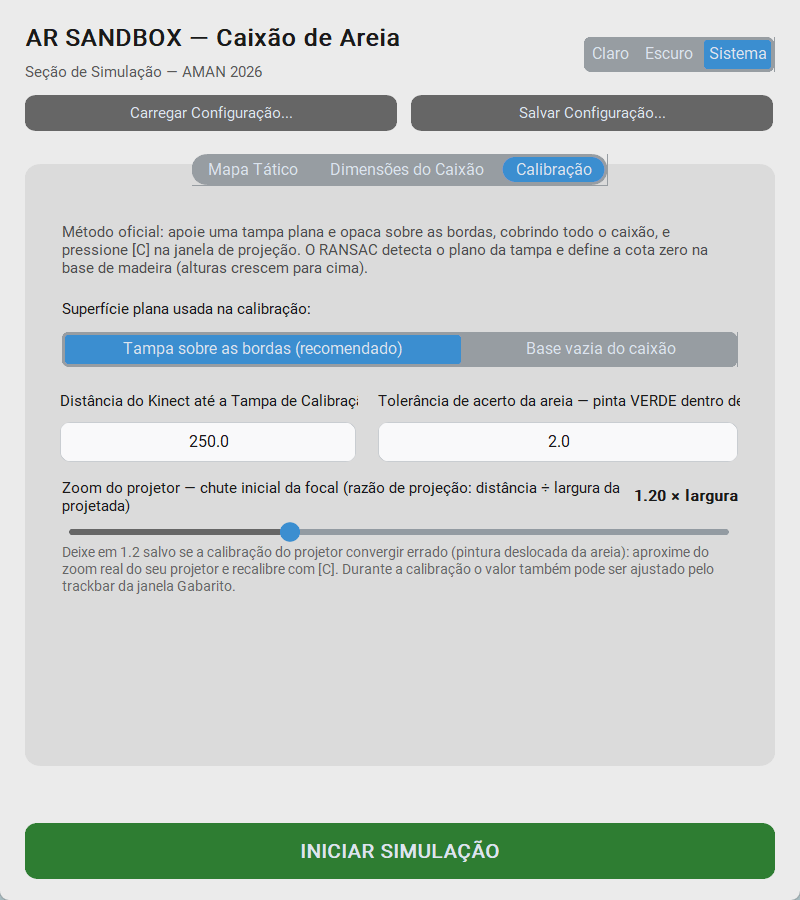
\includegraphics[width=0.75\textwidth]{img/gui_configuracao.png}
\caption{Interface gráfica de configuração inicial (CustomTkinter),
aba ``Calibração'': modo de calibração (tampa/base), distância do
Kinect à superfície de referência, tolerância de aceitação e o fator
inicial de zoom do projetor.}
\label{fig:gui-config}
\end{figure}

\subsection{Saída temporária de calibração: o tabuleiro quadriculado}
\label{subsec:saida-tabuleiro}

Durante a etapa opcional de calibração empírica do projetor
(via \texttt{calibrar\_projetor}, Seção~\ref{subsec:calib-empirica-projetor}), a janela
\texttt{Projecao\_Areia} deixa temporariamente de exibir a
malha de cores e passa a projetar um padrão de tabuleiro de
xadrez (\texttt{gerar\_imagem\_tabuleiro}) sobre a superfície de
referência. Essa saída é usada apenas enquanto dura a rotina de
calibração: uma câmera captura o tabuleiro projetado, a função
\texttt{encontrar\_cantos\_tabuleiro} detecta os cantos internos na
imagem capturada e \texttt{cv2.calibrateCamera} estima, por
otimização não linear, os parâmetros intrínsecos do projetor a partir
das correspondências entre cantos conhecidos e cantos detectados. Um
\textit{trackbar} de ajuste do fator de zoom/\textit{throw ratio}
(``\texttt{Zoom proj~x100}'') é exibido na janela \texttt{Gabarito\_MDE}
durante essa etapa, permitindo ao operador corrigir o chute inicial da
distância focal caso a otimização convirja para um mínimo local
incorreto. Encerrada a calibração — com sucesso ou por cancelamento —,
a janela \texttt{Projecao\_Areia} volta a exibir exclusivamente a
malha de cores. Este é, portanto, um mecanismo de depuração e
calibração assistida, e não uma saída destinada ao uso operacional
corrente do sistema; na configuração padrão, o sistema opera com os
parâmetros de projeção obtidos analiticamente
(Seção~\ref{sec:passo4}), e a rotina de tabuleiro permanece disponível
como caminho alternativo, já coberto pela suíte de testes
(Capítulo~\ref{cap:resultados}).

\section{Padrões de Projeto Aplicados}
\label{sec:patterns}

A Tabela~\ref{tab:patterns} elenca os padrões de projeto de
Gamma et al.~\citeonline{gamma1995design} identificados na implementação, e o
restante desta seção explica o propósito de cada um.

\begin{table}[!ht]
\centering
\caption{Padrões de projeto aplicados.}
\label{tab:patterns}
\begin{tabular}{lll}
\toprule
\textbf{Padrão} & \textbf{Onde} & \textbf{Propósito} \\
\midrule
Strategy + Fallback & \texttt{KinectSensor} & Seleção transparente de \textit{driver} \\
Adapter             & \texttt{AdaptadorMDE} & Isolar formato GeoTIFF da interface \\
State Machine       & \texttt{main.py}      & Controle determinístico do fluxo \\
Observer (Callback) & \texttt{main.py}      & Eventos de \emph{mouse} desacoplados \\
\bottomrule
\end{tabular}
\end{table}

\begin{description}
    \item[Strategy + \textit{Fallback} (\texttt{KinectSensor}).] Cada
          backend de captura (PyKinect2, Open3D, \texttt{freenect},
          simulação) implementa a mesma interface de
          \texttt{capturar\_nuvem()}, encapsulando um algoritmo de
          aquisição intercambiável — a essência do padrão
          \textit{Strategy}. A particularidade deste projeto é compor
          o \textit{Strategy} com uma cadeia de fallback
          (Seção~\ref{subsec:fallback}): em vez de o cliente escolher
          explicitamente a estratégia, o próprio construtor de
          \texttt{KinectSensor} tenta cada uma em ordem de preferência
          até que uma tenha sucesso, tornando a seleção do
          \textit{driver} transparente ao restante do sistema —
          \texttt{main.py} chama sempre o mesmo método, qualquer que
          seja o backend efetivamente ativo.
    \item[Adapter (\texttt{AdaptadorMDE}).] O formato de arquivo
          GeoTIFF, a biblioteca \texttt{rasterio} e a convenção de
          eixos cartográficos são detalhes de implementação que o
          restante do sistema não deveria conhecer. A classe
          \texttt{AdaptadorMDE} adapta essa interface heterogênea a um
          único método uniforme, \texttt{obter\_z\_alvo(x, y)}, que
          devolve a altura de referência em coordenadas físicas da
          mesa — seja a origem um GeoTIFF real, seja um mapa sintético
          de \textit{fallback} (Cubo Central ou Morro Gaussiano).
    \item[\textit{State Machine} (\texttt{main.py}).] A execução é
          modelada como uma enumeração explícita de estados
          (Seção~\ref{sec:fsm}) com transições determinísticas
          disparadas por eventos de teclado. Esse padrão evita a
          alternativa comum de controlar o fluxo por variáveis
          booleanas soltas (\emph{flags}), que tendem a
          produzir estados inválidos ou inconsistentes à medida que o
          programa cresce; aqui, o estado corrente é sempre um único
          valor da enumeração \texttt{Estado}, tornando impossível,
          por construção, que o sistema esteja simultaneamente
          calibrando e em \textit{loop} de Realidade Aumentada.
    \item[\textit{Observer} via \textit{callback} (\texttt{main.py}).]
          Os eventos de \emph{mouse} (pressionar, arrastar, soltar os
          botões) são registrados por \texttt{cv2.setMouseCallback} e
          notificados de forma assíncrona à função de tratamento, que
          atualiza o estado persistente da areia virtual
          (Seção~\ref{sec:emulador}) sem que o \textit{loop} principal
          precise consultar ativamente (\emph{polling}) a posição do
          cursor a cada quadro — um desacoplamento típico do padrão
          \textit{Observer}, aqui implementado pelo mecanismo nativo
          de \textit{callbacks} do OpenCV em vez de uma hierarquia
          explícita de classes \textit{Subject}/\textit{Observer}.
\end{description}

\subsection{Cadeia de \textit{fallback} do sensor}
\label{subsec:fallback}

O construtor do \texttt{KinectSensor} executa, em ordem, quatro
tentativas de inicialização. A primeira que tiver sucesso é mantida; em
caso contrário, prossegue-se ao próximo nível. A
Figura~\ref{fig:fallback} esquematiza a cadeia.

\begin{figure}[!ht]
\centering
\begin{lstlisting}[language=, basicstyle=\ttfamily\footnotesize, frame=single]
1. PyKinect2 (SDK Microsoft - Kinect v2)        ---falhou--> 2
2. Open3D    (Azure Kinect / RealSense)         ---falhou--> 3
3. freenect  (Kinect v1 / libfreenect)          ---falhou--> 4
4. SIMULACAO (grade persistente + pa virtual)   <-- sempre OK
\end{lstlisting}
\caption{Cadeia de \textit{fallback} do \texttt{KinectSensor}.}
\label{fig:fallback}
\end{figure}

A garantia operacional fundamental é que o sistema nunca falha
catastroficamente por ausência de hardware: o quarto nível
(Simulação) é puramente computacional e não depende de
quaisquer recursos externos. Garantia análoga aplica-se ao
\texttt{AdaptadorMDE}: na ausência ou falha de leitura do GeoTIFF, é
gerada uma superfície gaussiana sintética que assegura visualização
significativa para a audiência.

% =====================================================================
% cap-03-motor-matematico.tex — Capítulo 4: Motor Matemático
% =====================================================================

\chapter{Motor Matemático}
\label{cap:motor}

Este capítulo formaliza o \textit{pipeline} matemático que transforma
uma nuvem bruta de pontos do sensor Kinect em uma malha de quadrados
coloridos sobre a areia. Cada uma das quatro etapas é apresentada com
rigor algébrico e relacionada à sua implementação no módulo
\texttt{motor\_caixao\_areia.py}.

\section{Passo 1 — Ajuste de Plano: RANSAC seguido de SVD}
\label{sec:passo1}

Dada uma nuvem de $N$ pontos $\{\mathbf{p}_i\}_{i=1}^{N} \subset
\mathbb{R}^{3}$ capturados pelo Kinect sobre a superfície plana de
referência (a tampa apoiada sobre o caixão, ou a base de madeira vazia),
o problema é determinar o plano $\Pi: ax + by + cz + d = 0$ que melhor
se ajusta a essa superfície. O campo de visão do Kinect, contudo, é mais
largo que a área útil do caixão: a nuvem capturada inclui também a
moldura de madeira, o piso ao redor e ruído da sala — pontos que não
pertencem ao plano de referência e que distorceriam um ajuste de
mínimos quadrados ingênuo. Por isso a calibração oficial
(\texttt{main.\_executar\_calibracao}) combina dois métodos em
sequência: primeiro o RANSAC isola o maior subconjunto de
pontos coplanares (Seção~\ref{subsec:ransac}); em seguida, o
SVD refina a normal com precisão sub-milimétrica, mas apenas
sobre esse subconjunto de \emph{inliers}.

\subsection{Isolamento de inliers por RANSAC}

A função \texttt{ajustar\_plano\_ransac()} executa $n_{\text{iter}} =
1000$ iterações por padrão. A cada iteração, sorteia-se uma trinca de
pontos, constrói-se o plano candidato que passa por eles e contam-se os
\emph{inliers}: pontos da nuvem completa cuja distância ao plano
candidato é inferior a $d_{\text{in}} = 0{,}03$~m (3~cm). O plano
vencedor é o que acumula o maior número de inliers ao longo das
iterações. Se a fração de inliers do plano vencedor for inferior a
$30\,\%$ da nuvem, a função levanta \texttt{RuntimeError} — sintoma de
que a superfície de referência não domina o campo de visão do sensor
(tampa mal posicionada, por exemplo).

\subsection{Refinamento por SVD}

A solução clássica de mínimos quadrados procede em três etapas sobre o
conjunto de inliers identificado pelo RANSAC (e apenas sobre ele).
Primeiro, calcula-se o centroide e a matriz centralizada
\begin{equation}
\bar{\mathbf{p}} = \frac{1}{N} \sum_{i=1}^{N} \mathbf{p}_i,
\qquad
M = \begin{bmatrix}
(\mathbf{p}_1 - \bar{\mathbf{p}})^{T} \\
\vdots \\
(\mathbf{p}_N - \bar{\mathbf{p}})^{T}
\end{bmatrix} \in \mathbb{R}^{N \times 3}.
\end{equation}

Em seguida, aplica-se a decomposição em valores singulares
$M = U \Sigma V^{T}$ com $\Sigma = \text{diag}(\sigma_1, \sigma_2,
\sigma_3)$ e $\sigma_1 \geq \sigma_2 \geq \sigma_3 \geq 0$. O vetor
normal procurado é a última linha de $V^{T}$:
\begin{equation}
\mathbf{n} = V^{T}_{[3,:]}.
\end{equation}

Finalmente, o coeficiente $d$ é calculado pela substituição do
centroide na equação do plano: $d = -\mathbf{n} \cdot \bar{\mathbf{p}}$.
Por convenção, exige-se que $n_z > 0$ (vetor apontando para cima, em
direção ao Kinect); caso contrário, $\mathbf{n}$ é negado.

A função \texttt{ajustar\_plano\_svd()} encapsula esse procedimento e é
coberta por quatro testes unitários que verificam (i) unicidade da
normal, (ii) plano horizontal $z = 5$, (iii) plano inclinado e
(iv) exceção para $N < 3$. A função \texttt{ajustar\_plano\_ransac()},
que aplica o RANSAC descrito acima e delega o refinamento a
\texttt{ajustar\_plano\_svd()} sobre os inliers, é coberta por cinco
testes unitários adicionais (classe \texttt{TestRANSAC}), incluindo o
cenário motivador da especificação — uma nuvem sintética com moldura e
piso como \textit{outliers} ao redor da tampa — e a verificação de que
o refinamento final usa exclusivamente os inliers selecionados.

\section{Passo 2 — Construção da Base da Mesa}
\label{sec:passo2}

A normal $\mathbf{n}$ define inequivocamente o eixo $Z_{\text{mesa}}$,
mas a base ortonormal completa requer dois eixos adicionais $X_{\text{mesa}}$
e $Y_{\text{mesa}}$ ortogonais entre si e a $\mathbf{n}$. A escolha
desses eixos é livre a menos de rotação em torno da normal; adotamos a
convenção mais simples possível, baseada em uma semente padrão.

O algoritmo é o seguinte:

\begin{enumerate}
    \item $Z_{\text{mesa}} \leftarrow \mathbf{n} / \|\mathbf{n}\|$;
    \item Escolhe-se uma semente $\mathbf{s} = (1, 0, 0)^{T}$. Se
          $|\mathbf{s} \cdot Z_{\text{mesa}}| \geq 0{,}9$ (semente
          quase paralela à normal), substitui-se por $(0, 1, 0)^{T}$;
    \item Aplica-se Gram-Schmidt:
          $X_{\text{mesa}} = \dfrac{\mathbf{s} - (\mathbf{s} \cdot Z_{\text{mesa}}) Z_{\text{mesa}}}{\| \mathbf{s} - (\mathbf{s} \cdot Z_{\text{mesa}}) Z_{\text{mesa}} \|}$;
    \item Calcula-se $Y_{\text{mesa}} = Z_{\text{mesa}} \times
          X_{\text{mesa}}$, garantindo automaticamente um sistema
          dextrogiro.
\end{enumerate}

A ortonormalidade do conjunto $\{X_{\text{mesa}}, Y_{\text{mesa}},
Z_{\text{mesa}}\}$ — isto é, $X \cdot Y = X \cdot Z = Y \cdot Z = 0$ e
$\|X\| = \|Y\| = \|Z\| = 1$ — é assegurada por testes unitários
dedicados (\texttt{TestConstruirBase}).

\section{Passo 3 — Transformação Afim 4$\times$4}
\label{sec:passo3}

A transformação $T \in \mathbb{R}^{4 \times 4}$ que leva pontos do
referencial do Kinect ao referencial da mesa empilha os eixos da mesa
como linhas da matriz de rotação:
\begin{equation}
R = \begin{bmatrix}
X_{\text{mesa}}^{T} \\
Y_{\text{mesa}}^{T} \\
Z_{\text{mesa}}^{T}
\end{bmatrix},
\qquad
\mathbf{t} = -R \, \bar{\mathbf{p}},
\qquad
T = \begin{bmatrix} R & \mathbf{t} \\ \mathbf{0}^{T} & 1 \end{bmatrix}.
\end{equation}

\noindent A propriedade fundamental dessa construção é que, para
qualquer ponto $\mathbf{p}$ pertencente ao plano da mesa, a coordenada
transformada $z_{\text{mesa}} = 0$ — isto é, o plano da mesa torna-se o
plano $XY$ do novo sistema. Essa invariante é verificada pelo teste
\texttt{TestMatrizTransformacao}.

\subsection{Composição com $T_{\text{shift}}$ — centro lógico e cota zero na base}
\label{subsec:T-shift}

A matriz $T$ acima leva o centroide $\bar{\mathbf{p}}$ do plano
detectado à origem $(0, 0, 0)$. Entretanto, a convenção interna
de discretização e renderização (Capítulo~\ref{cap:rendering}) adota a
mesa como o domínio $[0, L_x] \times [0, L_y] \times [0, h_{\max}]$, com
a origem $XY$ em um canto e a cota $Z = 0$ fixada na base
de madeira do caixão (alturas de areia sempre positivas, crescendo
para cima). Sem ajuste em $XY$, metade dos pontos da nuvem (aqueles com
$x < 0$ ou $y < 0$) seria projetada fora do domínio e colapsada
pelo \texttt{clip} nas células de borda da grade — um defeito
observado em ensaio preliminar de campo, no qual a projeção exibia
apenas um pequeno retângulo correspondente ao quadrante positivo. E sem
ajuste em $Z$, a cota zero coincidiria com o plano de calibração
em vez da base do caixão — o que é apenas correto quando esse plano é a
própria base (modo base vazia), mas não quando ele é a tampa
apoiada $h_{\max}$ acima dela (modo tampa, oficial).

A solução, identificada e corrigida durante a fase de validação, é
compor $T$ com uma translação $T_{\text{shift}}$ que (i) desloca o
centroide para o centro lógico da mesa em $XY$ e (ii) desce a origem em
$Z$ até a base do caixão sempre que o plano de calibração for a tampa:
\begin{equation}
\label{eq:T-shift}
T_{\text{shift}} =
\begin{bmatrix}
1 & 0 & 0 & L_x / 2 \\
0 & 1 & 0 & L_y / 2 \\
0 & 0 & 1 & \delta_{\text{tampa}} \, h_{\max} \\
0 & 0 & 0 & 1
\end{bmatrix},
\qquad
T_{\text{final}} = T_{\text{shift}} \cdot T,
\end{equation}

\noindent onde $\delta_{\text{tampa}} = 1$ no modo tampa e
$\delta_{\text{tampa}} = 0$ no modo base vazia. Após essa composição, o
ponto físico que se encontra exatamente sob o sensor (centroide do
plano detectado) cai em $(L_x/2,\, L_y/2,\, \delta_{\text{tampa}}
h_{\max})$: no modo tampa, na cota $h_{\max}$ (o topo do caixão); no
modo base, na cota $0$ (o fundo, que é o próprio plano de
calibração). Em ambos os casos, a nuvem ocupa naturalmente $[0, L_x]
\times [0, L_y]$ em $XY$ e a base de madeira corresponde sempre a
$Z_{\text{mesa}} = 0$, independentemente do modo de calibração
escolhido. Adicionalmente, a função \texttt{discretizar\_nuvem\_em\_grade()}
aplica um filtro \texttt{dentro} que descarta pontos cujas
coordenadas $XY$ extrapolem o domínio físico da mesa, o que é típico do
campo de visão do Kinect montado a 2,5~m (FOV horizontal de
aproximadamente 70° cobre uma área maior do que a mesa).

Como validação de sanidade, antes de compor $T_{\text{shift}}$
o sistema compara a distância medida sensor–plano ($-\bar{p}_z$, uma
vez que $Z$ cresce em direção ao sensor no referencial original) com a
distância informada pelo operador na interface gráfica — a distância ao
plano da tampa no modo tampa, ou essa mesma distância somada a
$h_{\max}$ no modo base. Divergências acima de 15~cm abortam a
calibração com uma mensagem diagnóstica, protegendo contra tampa mal
posicionada ou erro de digitação nos campos físicos da mesa.

\section{Passo 4 — Projeção 3D$\to$2D pelo Modelo de Tsai}
\label{sec:passo4}

Os vértices da malha de quadrados (Capítulo~\ref{cap:rendering}) são
projetados do referencial 3D da mesa para o plano 2D do projetor pela
fórmula geral~\eqref{eq:pinhole}, com distorções óticas residuais
$(k_1, k_2, p_1, p_2, k_3)$ encapsuladas pela função
\texttt{cv2.projectPoints} do OpenCV.

Em modo simulação e em modo real, os parâmetros
intrínsecos e extrínsecos são configurados de forma a mapear o domínio
físico $[0, L_x] \times [0, L_y]$ na janela de projeção. Adotando uma
distância virtual da câmera $d_{\text{cam}} = 10$~m, $\mathbf{t}_{\text{ext}} =
(0, 0, d_{\text{cam}})^{T}$ e $R_{\text{ext}} = I_3$, obtém-se
\begin{equation}
\label{eq:fxfy-virtual}
f_x = \frac{W \cdot d_{\text{cam}}}{L_x}, \qquad
f_y = \frac{H \cdot d_{\text{cam}}}{L_y},
\qquad (c_x, c_y) = (0, 0),
\end{equation}

\noindent onde $(W, H)$ é a resolução do projetor. Substituindo em
\eqref{eq:pinhole}, vê-se que o ponto $(x, y, 0)$ projeta-se exatamente
em
\begin{equation}
u = \frac{W}{L_x} \, x, \qquad v = \frac{H}{L_y} \, y,
\end{equation}

\noindent o que é precisamente o mapeamento desejado de
$[0, L_x] \times [0, L_y]$ para $[0, W] \times [0, H]$. Essa parametrização
é compartilhada pelos dois modos de operação, o que simplifica a
calibração e elimina assimetrias entre simulação e hardware real. Como
o projetor é montado fisicamente alinhado — apontando reto para baixo,
centrado sobre a mesa —, esses parâmetros podem ser deduzidos
analiticamente, sem necessidade de um procedimento de estimação
experimental.

A Tabela~\ref{tab:intrinsecos-projetor} instancia a
Equação~\eqref{eq:fxfy-virtual} com os valores efetivamente usados
pelo sistema: a resolução de projeção padrão
(\texttt{RESOLUCAO\_PROJETOR}, fixa no código) e a distância virtual
$d_{\text{cam}} = 10$~m adotada em \texttt{main.py}, aplicadas à mesa
física de referência deste trabalho ($1,5~\text{m} \times
1,5~\text{m}$, Capítulo~\ref{cap:rendering}).

\begin{table}[!ht]
\centering
\caption{Parâmetros intrínsecos da câmera virtual do projetor (modelo analítico da Equação~\eqref{eq:fxfy-virtual}), instanciados para a mesa física de referência deste trabalho.}
\label{tab:intrinsecos-projetor}
\begin{tabular}{ll}
\toprule
\textbf{Parâmetro} & \textbf{Valor} \\
\midrule
Resolução do projetor $(W, H)$          & $640 \times 480$ pixels \\
Distância virtual da câmera $d_{\text{cam}}$ & $10{,}00$ m \\
Dimensões da mesa $(L_x, L_y)$          & $1{,}50 \times 1{,}50$ m \\
Distância focal $f_x$                   & $4\,266{,}67$ pixels \\
Distância focal $f_y$                   & $3\,200{,}00$ pixels \\
Centro óptico $(c_x, c_y)$              & $(0{,}00,\; 0{,}00)$ pixels \\
\bottomrule
\end{tabular}
\end{table}

Ao contrário dos parâmetros intrínsecos do Kinect
(Tabela~\ref{tab:intrinsecos}), que são uma especificação fixa do
fabricante do sensor, $f_x$ e $f_y$ do projetor não são uma constante
de hardware: dependem das dimensões físicas da mesa configuradas pelo
operador na inicialização do sistema (Apêndice~\ref{ap:roteiro}), já
que a Equação~\eqref{eq:fxfy-virtual} os deriva justamente dessas
dimensões. Os valores acima instanciam essa equação para a mesa de
referência ($1,5~\text{m} \times 1,5~\text{m}$) usada em todos os
ensaios e testes deste trabalho; $W$, $H$ e $d_{\text{cam}}$, por sua
vez, são constantes do sistema, fixas independentemente da mesa
configurada.

\subsection{Calibração empírica alternativa do projetor (tabuleiro de xadrez)}
\label{subsec:calib-empirica-projetor}

Caso a premissa de alinhamento físico não se sustente — projetor
montado com alguma inclinação residual, por exemplo —, o sistema
disponibiliza um caminho alternativo de estimação empírica dos
parâmetros de Tsai, no qual a etapa de otimização que o artigo original
de Tsai~\citeonline{tsai1987versatile} descreve é de fato executada. A
função \texttt{gerar\_imagem\_tabuleiro()} produz um padrão de
tabuleiro de xadrez com cantos internos em coordenadas conhecidas do
projetor; essa imagem é projetada temporariamente na janela
\texttt{Projecao\_Areia} sobre a superfície de referência ainda no
lugar (Seção~\ref{sec:saidas}). Uma câmera RGB captura o tabuleiro
projetado; \texttt{encontrar\_cantos\_tabuleiro()} localiza os cantos
na imagem capturada via \texttt{cv2.findChessboardCorners}; e
\texttt{cantos\_rgb\_para\_pontos\_mesa()} converte cada canto para uma
coordenada 3D no referencial da mesa, por \textit{back-projection}
(Equação~\eqref{eq:backproj}) seguida de $T_{\text{final}}$. Com as
correspondências 3D~$\leftrightarrow$~2D resultantes,
\texttt{calibrar\_projetor()} invoca \texttt{cv2.calibrateCamera} para
estimar $f_x, f_y, c_x, c_y$ e os coeficientes de distorção por
otimização não linear, a partir de um chute inicial de focal
configurável (fator ``\textit{throw ratio}'', padrão $1{,}2 \times$ a
largura do projetor em pixels — exposto ao operador por um controle
deslizante na GUI e por um \textit{trackbar} na janela
\texttt{Gabarito\_MDE} durante a calibração, permitindo corrigi-lo caso
a otimização convirja para um mínimo local incorreto). Esse caminho
alternativo é exercitado pelas classes de teste
\texttt{TestCalibracaoProjetorOpenCV}, \texttt{TestGeracaoTabuleiro},
\texttt{TestCantosParaPontosMesa} e
\texttt{TestPipelineCalibracaoProjetor} (Capítulo~\ref{cap:resultados}),
mas permanece inativo por padrão: a configuração corrente do
sistema opera com os parâmetros analíticos da
Equação~\eqref{eq:fxfy-virtual}, reservando a rotina empírica para o
cenário de montagem não idealizada.

\section{Discussão — RANSAC e SVD: uma composição deliberada}
\label{sec:discussao-svd}

Uma versão anterior deste trabalho empregava SVD puro, sem RANSAC, para
o ajuste de plano, sob a premissa de que a nuvem de calibração seria
capturada já livre de \textit{outliers}. A experimentação em
campo mostrou que essa premissa não se sustenta: o campo de visão do
Kinect~v2 é mais largo que a área útil do caixão de areia, de modo que
qualquer captura da superfície de referência inclui também a moldura de
madeira do caixão, o piso ao redor e ruído da sala. Um SVD aplicado
ingenuamente sobre a nuvem inteira minimiza a soma dos quadrados das
distâncias de \emph{todos} os pontos, inclusive desses outliers, o que
distorce sistematicamente a normal calculada. A solução adotada — e
validada nos ensaios de campo relatados no
Capítulo~\ref{cap:resultados} — não é substituir o SVD pelo RANSAC, mas
compor os dois, cada um explorando a etapa em que é mais forte:

\begin{itemize}
    \item O RANSAC (Seção~\ref{subsec:ransac}) é robusto a
          \textit{outliers} por construção: ele isola o maior
          subconjunto de pontos coplanares antes de qualquer ajuste
          numérico, funcionando mesmo com até $70\,\%$ da nuvem
          ocupada por pontos que não pertencem ao plano de referência
          (limite imposto por \texttt{min\_inliers\_ratio}~$= 0{,}3$);
    \item O SVD, aplicado apenas sobre os inliers
          selecionados pelo RANSAC, produz o estimador de mínimos
          quadrados \emph{ótimo} para esse subconjunto — mais preciso
          do que o plano obtido a partir de apenas três pontos
          amostrados em uma única iteração do RANSAC;
    \item A solução SVD é \emph{única} (a menos do sinal da normal,
          tratado por convenção), o que facilita a verificação por
          testes unitários com valores esperados \emph{hardcoded}
          sobre nuvens sintéticas 100\,\% coplanares — cenário em que
          o parâmetro \texttt{usar\_ransac=False} permanece disponível
          e suficiente, dispensando o custo das iterações RANSAC;
    \item Em contrapartida, o SVD isolado seria \emph{insuficiente}
          para o cenário real da tampa: sem a etapa de RANSAC, a
          normal calculada é sistematicamente puxada na direção dos
          outliers, produzindo o mesmo artefato de projeção deslocada
          relatado nos ensaios preliminares de campo
          (Seção~\ref{subsec:T-shift}).
\end{itemize}

\noindent A escolha entre os dois regimes é, portanto, guiada pela
origem dos dados: SVD puro para nuvens sintéticas já garantidamente
coplanares (a maioria dos testes unitários do motor matemático); RANSAC
seguido de SVD para qualquer nuvem capturada por hardware real, na qual
a presença de outliers geométricos é a regra, não a exceção.

\noindent Essa decisão é validada empiricamente: a suíte de 83 testes
unitários do motor matemático passa integralmente, incluindo os cinco
casos dedicados especificamente ao RANSAC (\texttt{TestRANSAC}) e os
oito casos da calibração pela tampa (\texttt{TestCalibracaoTampa}), com
as constantes algébricas explicitadas na própria suíte.

% =====================================================================
% cap-04-renderizacao.tex — Capítulo 5: Renderização e Emulador Interativo
% =====================================================================

\chapter{Renderização por Malha Discretizada e Emulador Interativo}
\label{cap:rendering}

Este capítulo descreve a estratégia de renderização adotada para
projetar, em tempo real, o \emph{feedback} visual sobre a areia, e
detalha o emulador interativo que permite a operação do sistema sem o
sensor Kinect físico.

\section{Motivação para a Discretização em Malha}
\label{sec:motiv-malha}

A primeira versão experimental do sistema projetava \emph{diretamente}
cada ponto da nuvem do Kinect como um \emph{pixel} colorido. Essa
abordagem revelou três deficiências severas:

\begin{enumerate}
    \item \textbf{Buracos visuais.} A densidade de pontos da nuvem é
          insuficiente para preencher continuamente a área projetada,
          resultando em uma textura ``pontilhada'' que prejudica a
          legibilidade do \textit{feedback}.
    \item \textbf{Ruído pixelizado.} O ruído do sensor produz cores
          oscilantes pixel a pixel, gerando uma imagem trêmula e
          desconfortável visualmente.
    \item \textbf{Custo computacional.} A invocação de
          \texttt{cv2.projectPoints} ou de equivalente para cada ponto
          individual é ineficiente em $\Theta(N)$.
\end{enumerate}

A solução proposta substitui a renderização pontual por uma
\textbf{discretização em malha regular}. Os pontos são agregados em
células retangulares, cada célula é classificada por uma única cor e
desenhada como um \emph{polígono preenchido} via
\texttt{cv2.fillPoly}.

\section{Definição Formal da Malha}
\label{sec:malha}

O domínio físico da mesa $[0, L_x] \times [0, L_y]$ é particionado em
uma malha regular de $N_x \times N_y$ células retangulares (por padrão
$N_x = N_y = 30$, totalizando 900 células). Cada célula $C_{i,j}$,
com $i \in \{0, \ldots, N_y - 1\}$ e $j \in \{0, \ldots, N_x - 1\}$,
ocupa o subdomínio
\begin{equation}
C_{i,j} = \big[ j \Delta x,\; (j+1) \Delta x \big]
        \times \big[ i \Delta y,\; (i+1) \Delta y \big],
\end{equation}

\noindent com $\Delta x = L_x / N_x$ e $\Delta y = L_y / N_y$. Para a
mesa de 1,5~m$\,\times\,$1,5~m com 30$\,\times\,$30 células, cada célula
mede precisamente 5~cm$\,\times\,$5~cm. A malha de células gera
$(N_x + 1)(N_y + 1) = 31 \times 31 = 961$ vértices distintos.

\section{Agregação Espacial e Filtragem de Ruído}
\label{sec:agregacao}

Para cada célula $C_{i,j}$ define-se o conjunto de pontos da nuvem que
nela se encontram:
\begin{equation}
\mathcal{P}_{i,j} = \big\{ \mathbf{p}_k = (x_k, y_k, z_k) :
    (x_k, y_k) \in C_{i,j} \big\},
\end{equation}

\noindent e a altura representativa da célula é a média aritmética dos
valores $Z$ dos pontos contidos:
\begin{equation}
\bar{Z}^{\text{real}}_{i,j} = \frac{1}{|\mathcal{P}_{i,j}|}
        \sum_{\mathbf{p}_k \in \mathcal{P}_{i,j}} z_k.
\end{equation}

Sob a hipótese de ruído gaussiano independente e identicamente
distribuído com desvio padrão $\sigma$, o desvio padrão da estimativa
da média é
\begin{equation}
\sigma_{\bar{Z}_{i,j}} = \frac{\sigma}{\sqrt{|\mathcal{P}_{i,j}|}},
\end{equation}

\noindent o que evidencia a \emph{filtragem estatística} obtida pela
agregação. Tipicamente, com a resolução de profundidade do Kinect~v2 e a
mesa coberta integralmente, cada célula recebe entre dezenas e centenas
de pontos, reduzindo o ruído em mais de uma ordem de grandeza.

A implementação é totalmente vetorizada via NumPy, dispensando laços
\textit{Python}. As somas e contagens por célula são acumuladas em
duas matrizes $N_y \times N_x$ pela função \texttt{numpy.add.at}.
Células sem pontos ($|\mathcal{P}_{i,j}| = 0$) são marcadas com
\texttt{NaN} e simplesmente \emph{não renderizadas} no
\textit{frame} corrente.

\section{Regra de Coloração}
\label{sec:cor}

O centro geométrico da célula $C_{i,j}$,
$\mathbf{c}_{i,j} = ((j + \tfrac{1}{2}) \Delta x, (i + \tfrac{1}{2}) \Delta y)$,
é usado para consultar a altura alvo do MDE:
$Z^{\text{MDE}}_{i,j} = \texttt{obter\_z\_alvo}(\mathbf{c}_{i,j})$.
A cor da célula segue então a regra parametrizada pela tolerância
$\tau$ (padrão: $\tau = 0{,}02$~m, equivalente a 2~cm):
\begin{equation}
\text{cor}(i, j) = \begin{cases}
\textbf{Vermelho} & \text{se } \bar{Z}^{\text{real}}_{i,j} > Z^{\text{MDE}}_{i,j} + \tau \\
\textbf{Azul}     & \text{se } \bar{Z}^{\text{real}}_{i,j} < Z^{\text{MDE}}_{i,j} - \tau \\
\textbf{Verde}    & \text{caso contrário}
\end{cases}
\end{equation}

\noindent A interpretação operacional é direta: \textbf{Vermelho}
indica excesso de areia (\emph{cavar}), \textbf{Azul} indica falta
(\emph{preencher}) e \textbf{Verde} indica conformidade com o MDE
dentro da tolerância (\emph{OK}).

\section{Projeção em Lote e Rasterização}
\label{sec:rasterizacao}

Os 961 vértices da malha 3D, todos com $Z = 0$ por estarem no plano da
mesa, são empilhados em uma única matriz $\mathbb{R}^{961 \times 3}$ e
projetados em um \emph{único} chamado a \texttt{cv2.projectPoints}, o
que corresponde a apenas \emph{uma} invocação de
\texttt{cv2.projectPoints} por \textit{frame}. Em seguida, cada célula
é desenhada como um quadrilátero preenchido pelos seus quatro vértices
projetados:
\begin{equation}
\text{quad}(i,j) = \big[ V_{i,j},\; V_{i,j+1},\; V_{i+1,j+1},\; V_{i+1,j} \big].
\end{equation}

\noindent O traçado é realizado por
\texttt{cv2.fillPoly(imagem, [quad], cor)}, que é uma rotina
otimizada nativamente em C++. O custo total de renderização por
\emph{frame} é, portanto, $O(N_x \cdot N_y)$ chamadas leves a
\texttt{fillPoly}, em vez dos $\Theta(N)$ pontos individuais da
abordagem ingênua.

\section{Emulador Interativo de Areia}
\label{sec:emulador}

\subsection{Estado persistente da areia virtual}

A classe \texttt{KinectSensor}, quando em modo simulação, mantém uma
matriz de alturas persistente $\mathbf{H} \in \mathbb{R}^{R \times R}$
(onde $R = 50$ é a resolução padrão), inicializada uniformemente em
$h_{\max} / 2 = 0{,}15$~m, simulando uma caixa preenchida com areia
nivelada na metade da profundidade máxima.

A cada chamada de \texttt{capturar\_nuvem()}, a função reconstrói a
nuvem $\{(x_j, y_i, H_{i,j})\}$ a partir do estado corrente da matriz
$\mathbf{H}$, refletindo imediatamente quaisquer modificações realizadas
pelo \emph{mouse}.

\subsection{Modelo gaussiano da pá virtual}

Ao receber um evento de \emph{mouse} na posição física $(x_m, y_m)$ da
mesa, o sistema atualiza $\mathbf{H}$ pela regra
\begin{equation}
H_{i,j}^{(t+1)} = \text{clip}\!\left(
H_{i,j}^{(t)} \pm \alpha \exp\!\left(
-\frac{(x_j - x_m)^2 + (y_i - y_m)^2}{2\sigma^2}
\right), 0, h_{\max} \right),
\end{equation}

\noindent com sinal $+$ ao preencher (botão direito) e $-$ ao cavar
(botão esquerdo). Os parâmetros padrão são $\alpha = 0{,}008$~m
(deslocamento por evento) e $\sigma = r/2 = 0{,}05$~m (raio de ação
$r = 0{,}10$~m).

A escolha do perfil gaussiano produz deformações suaves e visualmente
naturais, em contraste com escavações cilíndricas ou retangulares. Como
mais de 86\% da energia do operador concentra-se dentro do raio $r$
(integrando-se a gaussiana 2D até esse raio, obtém-se
$1 - e^{-2} \approx 0{,}865$), o controle ergonômico é direto.

\subsection{Mapeamento \textit{pixel}$\to$coordenada física}

O \textit{callback} de \emph{mouse}, registrado via
\texttt{cv2.setMouseCallback}, converte cada coordenada de \emph{pixel}
$(u, v)$ em coordenada física $(x_{\text{mesa}}, y_{\text{mesa}})$
proporcionalmente às dimensões correntes da janela
(\texttt{cv2.getWindowImageRect}):
\begin{equation}
x_{\text{mesa}} = \frac{u}{W_{\text{janela}}} \cdot L_x,
\qquad
y_{\text{mesa}} = \frac{v}{H_{\text{janela}}} \cdot L_y.
\end{equation}

\noindent O sistema trata graciosamente eventos fora da área da imagem
(simplesmente ignorados) e dimensões de janela inválidas (fallback à
resolução nominal do projetor). O \emph{callback} é silenciosamente
ignorado em modo real, evitando interferência com o sensor físico.

% =====================================================================
% cap-05-resultados.tex — Capítulo 6: Resultados e Validação
% =====================================================================

\chapter{Resultados e Validação}
\label{cap:resultados}

Este capítulo apresenta os resultados experimentais obtidos na
validação do sistema, organizados em cinco frentes: a estratégia de
testes automatizados (Seção~\ref{sec:tdd}), as evidências quantitativas
de corretude e reprodutibilidade — gráficos, cobertura de código,
comparação entre testes unitários e de ponta a ponta, e a discussão
transparente das limitações da validação física
(Seção~\ref{sec:evidencias}) —, a validação funcional do
\textit{pipeline} completo em simulação e em hardware real
(Seção~\ref{sec:funcional}), a discussão da correção do defeito de
calibração detectado em ensaio preliminar (Seção~\ref{sec:correcao}) e
a discussão dos principais \emph{trade-offs} de projeto
(Seção~\ref{sec:tradeoffs}).

\section{Estratégia de Testes Automatizados}
\label{sec:tdd}

A estabilidade matemática do motor foi assegurada pela adoção de
Test-Driven Development (TDD): cada função do módulo
\texttt{motor\_caixao\_areia.py} foi acompanhada por um conjunto de
testes unitários escritos previamente, com valores numéricos
\emph{hardcoded} cuja correção é verificável passo a passo. A suíte
cresceu ao longo do projeto à medida que novas etapas do
\textit{pipeline} foram implementadas — da versão inicial com 26 casos
(cobrindo apenas SVD, Gram-Schmidt, transformação afim, projeção Tsai e
regra de cor) até a suíte atual, com 83 testes. Para deixar
explícito \emph{o que} cada teste verifica, a Tabela~\ref{tab:tests}
agrupa as 22 classes em cinco frentes funcionais do \textit{pipeline},
em vez de listá-las na ordem em que aparecem no código-fonte.

\begin{table}[!ht]
\centering
\caption{Estrutura da suíte de testes unitários, por frente funcional (estado atual).}
\label{tab:tests}
\small
\begin{tabularx}{\textwidth}{@{}l X c@{}}
\toprule
\textbf{Classe} & \textbf{Componente verificado} & \textbf{Testes} \\
\midrule
\multicolumn{3}{@{}l}{\textbf{1. Calibração Kinect~$\to$~Mesa (RANSAC + SVD + Gram-Schmidt + $T_{\text{shift}}$)}} \\
\texttt{TestAjustePlano}             & SVD, normal unitária, equação do plano          & 4 \\
\texttt{TestRANSAC}                  & Isolamento de inliers, exceções, refinamento SVD & 5 \\
\texttt{TestGramSchmidt}             & Ortogonalidade, exceção paralelos               & 2 \\
\texttt{TestConstruirBase}           & Ortonormalidade dos eixos                       & 3 \\
\texttt{TestMatrizTransformacao}     & Identidade, translação, $z_{\text{mesa}} = 0$   & 3 \\
\texttt{TestCalibracaoTampa}         & Modos tampa/base, $T_{\text{shift}}$, cota zero & 8 \\
\texttt{TestPersistenciaCalibracao}  & \texttt{calibration\_data.json} (esquema v2)    & 6 \\
\emph{Subtotal} & & \emph{31} \\
\addlinespace
\multicolumn{3}{@{}l}{\textbf{2. Calibração Mesa~$\to$~Projetor (Tsai analítico e empírico)}} \\
\texttt{TestProjecaoTsai}            & Projeção \textit{pinhole} analítica             & 3 \\
\texttt{TestDeteccaoTabuleiro}       & Detecção de tabuleiro $7 \times 5$              & 2 \\
\texttt{TestGeracaoTabuleiro}        & Geração do padrão projetado                     & 2 \\
\texttt{TestCantosParaPontosMesa}    & \textit{Back-projection} dos cantos             & 2 \\
\texttt{TestCalibracaoProjetorOpenCV}& \texttt{cv2.calibrateCamera}, \texttt{solvePnP} & 6 \\
\texttt{TestPipelineCalibracaoProjetor} & Calibração empírica ponta a ponta            & 5 \\
\emph{Subtotal} & & \emph{20} \\
\addlinespace
\multicolumn{3}{@{}l}{\textbf{3. Captura e leitura de profundidade}} \\
\texttt{TestBackProjectionMesa}      & Pixel $\to$ ponto 3D da mesa                    & 4 \\
\texttt{TestLeituraRGBD}             & Importação condicional Open3D                   & 1 \\
\emph{Subtotal} & & \emph{5} \\
\addlinespace
\multicolumn{3}{@{}l}{\textbf{4. MDE de referência e regra de cor}} \\
\texttt{TestCuboCentral}             & Mapa sintético Cubo Central                     & 7 \\
\texttt{TestMorroGaussiano}          & Mapa sintético Morro Gaussiano                  & 4 \\
\texttt{TestColoracaoBGR}            & Regra Vermelho/Azul/Verde (escalar e vetorizada) & 10 \\
\emph{Subtotal} & & \emph{21} \\
\addlinespace
\multicolumn{3}{@{}l}{\textbf{5. Discretização, renderização e integração ponta a ponta}} \\
\texttt{TestDiscretizacaoGradeNegativa} & Filtro \texttt{dentro} do domínio             & 1 \\
\texttt{TestRenderizacaoGrade}       & Rasterização \texttt{cv2.fillPoly}              & 2 \\
\texttt{TestPipeline}                & Integração Passos 1+2                           & 2 \\
\texttt{TestFluxoAceitacao}          & Aceitação ponta a ponta (Seção~\ref{sec:aceitacao}) & 1 \\
\emph{Subtotal} & & \emph{6} \\
\midrule
\textbf{Total}                        & \multicolumn{2}{r}{\textbf{83}}                \\
\bottomrule
\end{tabularx}
\end{table}

\noindent Além da contagem de casos, a cobertura de código
(medida com \texttt{coverage.py} sobre os dois módulos que concentram
a lógica matemática) confirma que essa suíte exercita a maior parte do
código de produção: 91\% das linhas de
\texttt{motor\_caixao\_areia.py} e 48\% das linhas de
\texttt{mde\_cartografia.py} são executadas durante os testes
(75\% combinado). A lacuna em \texttt{mde\_cartografia.py}
concentra-se quase inteiramente no método \texttt{\_carregar()}, que lê
um arquivo GeoTIFF real via \texttt{rasterio} — caminho que a suíte
atual não exercita: todos os testes usam os mapas sintéticos (Cubo
Central ou Morro Gaussiano), mesmo havendo um GeoTIFF real versionado
no repositório (\texttt{25S51\_ZN.tif}, $5400 \times 3600$ pixels,
cobrindo uma faixa do sul do Brasil) que hoje não é referenciado nem
pela configuração padrão do sistema nem por qualquer caso de teste.
Essa lacuna é uma limitação conhecida e explícita da suíte, não uma
omissão silenciosa: a leitura de um GeoTIFF real permanece sem teste
automatizado dedicado, e sua correção — escrever um teste que carregue
\texttt{25S51\_ZN.tif} e valide a interpolação bilinear contra valores
conhecidos da grade — é uma melhoria de baixo custo e alto valor para
trabalhos futuros.

\subsection{Filosofia: transparência matemática}

Cada teste documenta, em comentário, a conta esperada passo a passo,
permitindo verificação independente. A título de exemplo, o teste
do plano horizontal $z = 5$ é resumido como:

\begin{lstlisting}[caption={Teste do plano horizontal — verificação manual.}, label=lst:test-plano]
# Pontos: (0,0,5), (1,0,5), (0,1,5), (1,1,5), (2,3,5)
# Centroide esperado: (0.8, 0.8, 5.0)
# Normal esperada:    (0, 0, 1)  -- plano horizontal
# d esperado:         -5
# Verificacao:  n . p + d = (0,0,1) . (0,0,5) + (-5) = 5 - 5 = 0  OK
\end{lstlisting}

A execução completa (\texttt{python -m unittest test\_motor\_caixao -v})
reporta 83 testes aprovados, nenhuma falha. O único teste
condicional da suíte, \texttt{TestLeituraRGBD}, é ignorado apenas em
ambientes sem a biblioteca Open3D instalada; no ambiente de validação
deste trabalho, Open3D estava presente e o teste foi executado
normalmente.

\subsection{Teste de aceitação de ponta a ponta}
\label{sec:aceitacao}

Além dos testes unitários por função, a classe
\texttt{TestFluxoAceitacao} reproduz, com nuvens de profundidade
sintéticas, o procedimento de aceitação físico usado para
validar o sistema perante a banca: (A) o caixão vazio é calibrado no
modo tampa; (B) o mapa alvo é o Cubo Central, que pede $+10$~cm no
terço central da mesa; (C) a base vazia, fora do cubo, deve ser
projetada em verde (a altura medida coincide com a cota zero
alvo); (D) o centro, ainda vazio, deve ser projetado em azul
(falta volume); (E) após a inserção de um cubo físico de 10~cm no
centro, o topo do cubo deve passar a ser projetado em verde, e
a base ao redor deve permanecer verde. O teste replica exatamente a
geometria \textit{pinhole} do sensor sintético e o mesmo caminho de
código do \texttt{main.py} (\texttt{profundidade\_para\_nuvem\_mesa}
$\to$ \texttt{transformar\_pontos} $\to$
\texttt{discretizar\_nuvem\_em\_grade} $\to$
\texttt{cor\_por\_diferenca\_vetorizado}), constituindo uma verificação
automatizada e reprodutível do cenário que, em campo, é demonstrado
fisicamente à banca com o caixão de areia real (Apêndice~A).

\section{Evidências Quantitativas de Corretude e Reprodutibilidade}
\label{sec:evidencias}

As seções anteriores descreveram \emph{o que} a suíte de testes cobre.
Esta seção tem um objetivo diferente e deliberadamente mais exigente:
reunir, em um único lugar, dados brutos, gráficos e trechos de código e
de saída de terminal reais que permitem a qualquer leitor
— sem precisar confiar na palavra dos autores — verificar
independentemente que o motor matemático do sistema funciona
corretamente. Nada nesta seção é hipotético: todos os números, tabelas
e gráficos foram gerados executando o código-fonte efetivamente
versionado no repositório, nas datas indicadas, e podem ser
reproduzidos por qualquer pessoa com Python 3.11+ e as dependências de
\texttt{requirements.txt} instaladas, com os dois comandos apresentados
na Seção~\ref{subsec:reprodutibilidade}.

\subsection{Funcionamento dos testes unitários}
\label{subsec:unitarios}

Um teste unitário, na suíte \texttt{test\_motor\_caixao.py}, segue
invariavelmente a mesma estrutura de três partes (\emph{arrange-act-assert}):
(1) constrói-se uma entrada sintética mínima — poucos pontos 3D, uma
imagem de tabuleiro gerada em memória, um pequeno JSON de calibração
— cujo resultado matematicamente correto é conhecido \emph{a priori}
e pode ser conferido manualmente, como exemplificado na
Listagem~\ref{lst:test-plano}; (2) a função de produção sob teste é
chamada exatamente como seria chamada por \texttt{main.py}, sem
\emph{mocks} do próprio algoritmo (apenas dependências externas
genuinamente indisponíveis em ambiente de CI, como o hardware Kinect,
são substituídas); (3) o resultado obtido é comparado ao valor
esperado com \texttt{assertAlmostEqual} (tolerância de ponto
flutuante) ou \texttt{numpy.testing.assert\_array\_equal}, e o teste
falha de forma explícita e localizada caso a conta não bata. Cada caso
de teste é independente dos demais — a classe \texttt{unittest.TestCase}
não compartilha estado mutável entre métodos — o que garante que a
ordem de execução não influencia o resultado e que uma eventual falha
aponta para exatamente uma função, nunca para uma interação obscura
entre testes.

A suíte não foi escrita de uma só vez ao final do projeto: ela cresceu
em paralelo com o próprio motor matemático, característica central da
metodologia TDD declarada na Seção~\ref{sec:tdd}. A
Figura~\ref{fig:crescimento-suite} traça essa evolução a partir do
histórico real de \emph{commits} do repositório que tocaram o arquivo
\texttt{test\_motor\_caixao.py}: de 26 testes na primeira versão
funcional (abril/2026) até os 83 testes atuais (agosto/2026), sem
nenhum retrocesso no total — evidência de que cada nova capacidade do
\textit{pipeline} (calibração por RANSAC, calibração empírica do
projetor, persistência em JSON, mapa Morro Gaussiano etc.) veio
acompanhada de sua própria verificação automatizada, em vez de testes
adicionados retroativamente apenas para efeito deste relatório.

\begin{figure}[!ht]
\centering
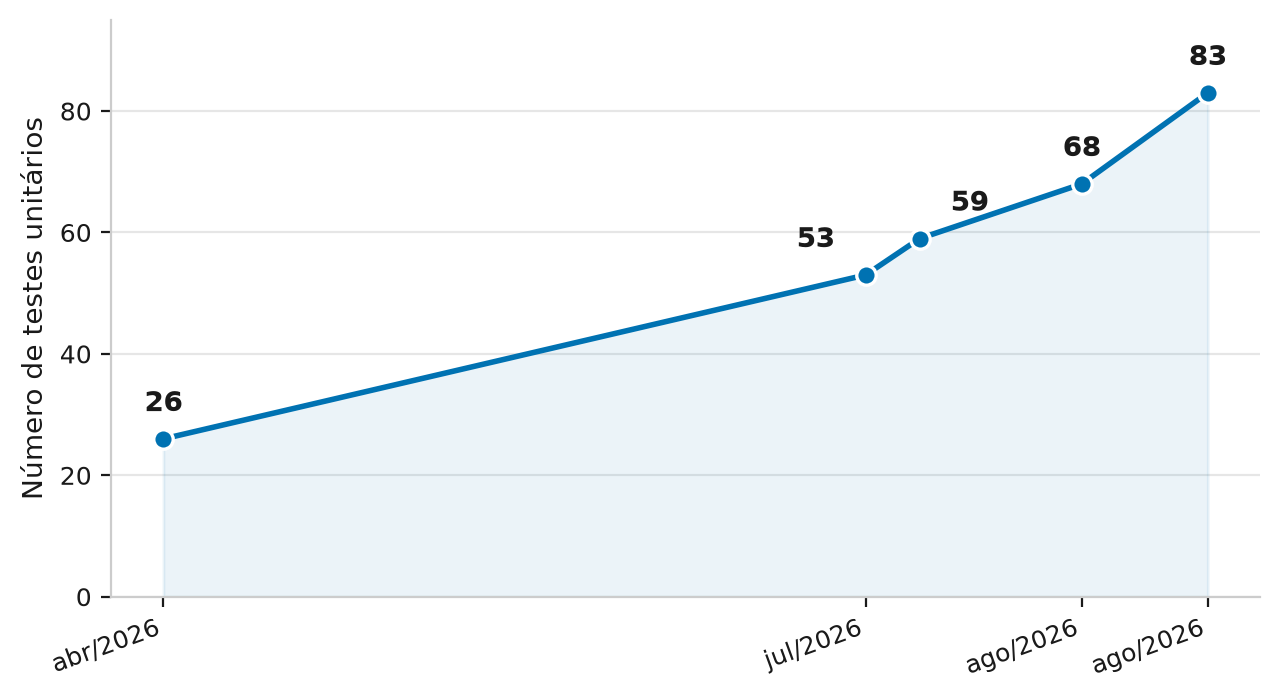
\includegraphics[width=0.75\textwidth]{img/grafico_crescimento_suite.png}
\caption{Crescimento do número de testes unitários ao longo do
histórico de \emph{commits} do repositório que modificaram
\texttt{test\_motor\_caixao.py} (dados extraídos de \texttt{git log}).}
\label{fig:crescimento-suite}
\end{figure}

A Figura~\ref{fig:testes-frente} traduz em gráfico a mesma distribuição
por frente funcional já detalhada na Tabela~\ref{tab:tests}, deixando
visualmente claro que nenhuma etapa do \textit{pipeline} — da
calibração geométrica à rasterização final — ficou sem cobertura de
teste dedicada.

\begin{figure}[!ht]
\centering
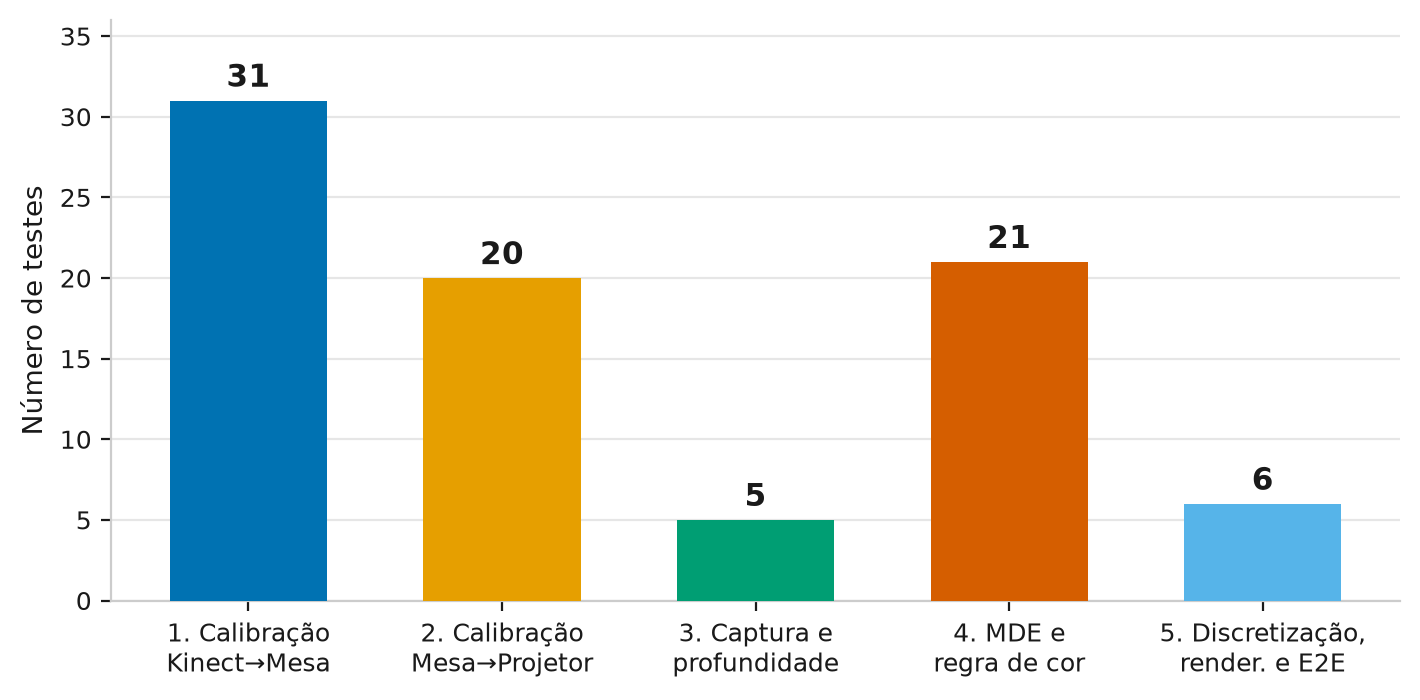
\includegraphics[width=0.85\textwidth]{img/grafico_testes_por_frente.png}
\caption{Distribuição dos 83 testes unitários pelas cinco frentes
funcionais do \textit{pipeline} (mesmos dados da Tabela~\ref{tab:tests}).}
\label{fig:testes-frente}
\end{figure}

A execução completa e literal, capturada diretamente do terminal no
ambiente de validação deste trabalho, é reproduzida na
Listagem~\ref{lst:saida-testes} — sem nenhuma edição além da omissão
das 83 linhas individuais \texttt{ok} por brevidade editorial (todas
presentes na execução real, cada uma identificando o teste
correspondente).

\begin{lstlisting}[caption={Saída real de \texttt{python -m unittest test\_motor\_caixao -v} no ambiente de validação.}, label=lst:saida-testes]
$ python -m unittest test_motor_caixao -v
test_plano_horizontal_z5 (test_motor_caixao.TestAjustePlano) ... ok
test_plano_inclinado_simples (test_motor_caixao.TestAjustePlano) ... ok
[... 79 testes intermediarios omitidos (todos "ok") ...]
test_pixel_verde_e_vermelho_em_celulas_distintas
    (test_motor_caixao.TestRenderizacaoGrade) ... ok

----------------------------------------------------------------------
Ran 83 tests in 2.264s

OK
\end{lstlisting}

\subsection{Cobertura de código: quanto do sistema é realmente exercitado}
\label{subsec:cobertura}

Contar testes prova apenas que a suíte existe; a cobertura de
linhas, medida com a ferramenta \texttt{coverage.py} instrumentando o
interpretador durante a execução da suíte, prova quanto do código de
produção é de fato exercitado por ela — isto é, quantas linhas
efetivamente rodam pelo menos uma vez sob teste, e não apenas quantas
funções têm algum caso associado. A Figura~\ref{fig:cobertura-modulos}
apresenta esses números para os dois módulos que concentram a lógica
matemática do sistema; a discussão qualitativa da lacuna em
\texttt{mde\_cartografia.py} (concentrada no carregamento de GeoTIFF
real, caminho não exercitado pela suíte sintética atual) já foi
apresentada na Seção~\ref{sec:tdd} e não é repetida aqui.

\begin{figure}[!ht]
\centering
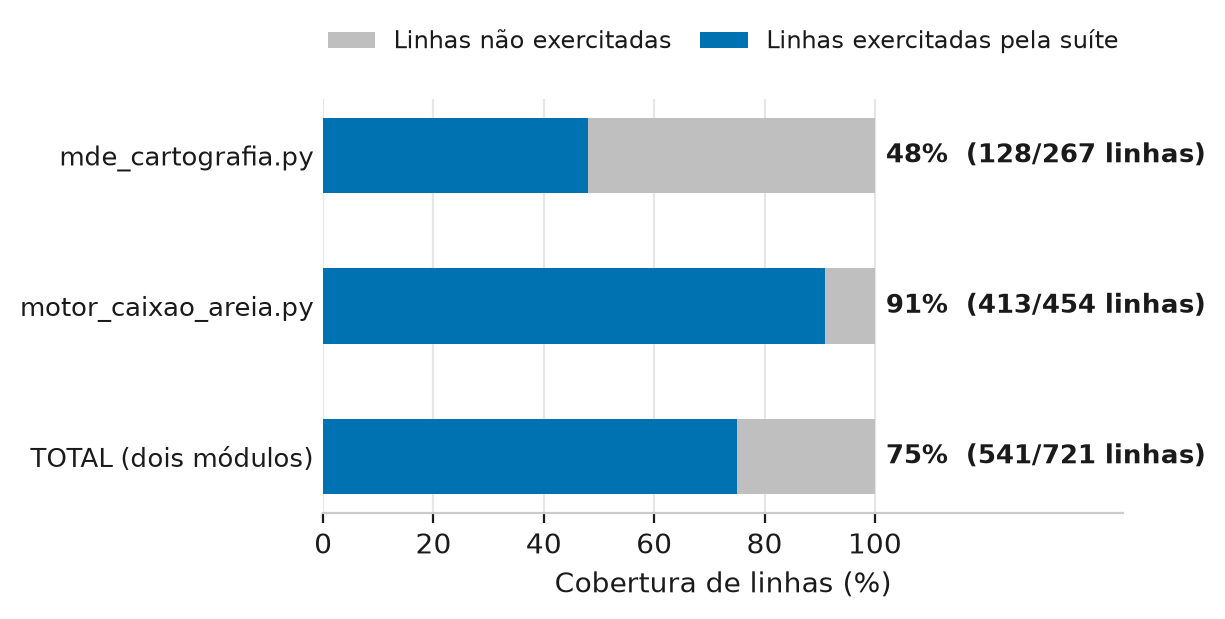
\includegraphics[width=0.8\textwidth]{img/grafico_cobertura.png}
\caption{Cobertura de linhas por módulo, medida com \texttt{coverage.py}
sobre a execução completa da suíte de testes.}
\label{fig:cobertura-modulos}
\end{figure}

A Listagem~\ref{lst:saida-cobertura} reproduz literalmente a saída do
comando \texttt{coverage report -m}, incluindo os números exatos de
linhas cobertas (\texttt{Stmts}) e não cobertas (\texttt{Miss}) por
módulo — os mesmos números usados para construir a
Figura~\ref{fig:cobertura-modulos}, sem qualquer arredondamento ou
seleção editorial.

\begin{lstlisting}[caption={Saída real de \texttt{coverage report -m}, medida sobre a suíte completa.}, label=lst:saida-cobertura]
Name                     Stmts   Miss  Cover   Missing
--------------------------------------------------------
mde_cartografia.py         267    139    48%   64-65, 70-72,
    76-77, 335-366, 378-484, 494, 557-565, 571, 577-579, 611,
    627-640, 664, 681-695, 726-772, 781, 791, 796, 801-803, 806-813
motor_caixao_areia.py      454     41    91%   164, 367, 523,
    696, 726, 799-808, 876, 979, 1036-1037, 1176, 1185,
    1221-1227, 1338, 1352, 1391-1417, 1431-1432, 1456, 1695, 1705
--------------------------------------------------------
TOTAL                      721    180    75%
\end{lstlisting}

\subsection{Testes unitários \textit{versus} testes de ponta a ponta}
\label{subsec:unit-vs-e2e}

Os dois estilos de teste presentes na suíte respondem a perguntas
diferentes e são complementares, não substitutos: um teste
unitário prova que uma peça isolada do motor matemático está correta;
um teste de ponta a ponta (\textit{end-to-end}, E2E) prova que as
peças, \emph{montadas na mesma ordem em que \texttt{main.py} as
monta}, produzem o comportamento correto quando compostas. A
Tabela~\ref{tab:unit-vs-e2e} resume as diferenças operacionais entre
os dois estilos, tais como efetivamente implementados na suíte.

\begin{table}[!ht]
\centering
\caption{Testes unitários \textit{versus} teste de ponta a ponta, na suíte atual.}
\label{tab:unit-vs-e2e}
\small
\begin{tabularx}{\textwidth}{@{}l X X@{}}
\toprule
\textbf{Dimensão} & \textbf{Teste unitário (82 casos)} & \textbf{Teste E2E (1 caso)} \\
\midrule
Exemplo & \texttt{TestGramSchmidt}, \texttt{TestProjecaoTsai}, \dots & \texttt{TestFluxoAceitacao} \\
Escopo & Uma única função de produção, isolada & Cadeia completa: captura $\to$ transformação $\to$ grade $\to$ MDE $\to$ cor \\
Entrada & Poucos pontos/valores artificiais, escolhidos a dedo & Nuvem de profundidade sintética de $512 \times 424$ pixels — os intrínsecos reais do Kinect~v2 (Tabela~\ref{tab:intrinsecos}), não um substituto simplificado — emulando um \textit{frame} Kinect completo \\
Oráculo (valor esperado) & Calculado manualmente, passo a passo (Listagem~\ref{lst:test-plano}) & Derivado do roteiro de aceitação físico da especificação (passos A--E, Apêndice~A) \\
Depende de outros módulos do sistema? & Não — isolamento deliberado & Sim, por construção: é exatamente isso que o teste verifica \\
Depende de hardware físico? & Não & Não (nuvem sintética; mesma geometria \textit{pinhole} do sensor real) \\
Tempo de execução & Tipicamente $< 5$~ms cada & $\approx 0{,}1$--$0{,}2$~s \\
O que uma falha indica & Um contrato matemático específico foi violado — regressão local, trivial de localizar & Uma quebra na \emph{integração} entre módulos, mesmo que cada peça isolada ainda passe — regressão sistêmica \\
\bottomrule
\end{tabularx}
\end{table}

O teste \texttt{TestFluxoAceitacao} (Listagem~\ref{lst:e2e-code} mostra
o método principal, extraído literalmente do código-fonte) reproduz os
cinco passos do roteiro de aceitação apresentado na
Seção~\ref{sec:aceitacao}: constrói uma nuvem de profundidade sintética
para o caixão vazio, calibra-a com a mesma rotina RANSAC~+~SVD usada em
produção (\texttt{semente\_rng=42}, fixa e determinística — a mesma
execução produz sempre o mesmo resultado, sem \emph{flakiness}),
verifica que a base vazia é projetada em verde e o terço central em
azul (passos C e D), sintetiza a inserção de um cubo físico de 10~cm no
centro alterando apenas a profundidade lida pelo sensor sintético, e
verifica que o topo do cubo passa a ser projetado em verde enquanto a
base ao redor permanece verde (passo E). Cada uma dessas verificações é
uma asserção \texttt{numpy.testing.assert\_array\_equal} sobre a cor
\emph{exata} (BGR) produzida pelo \textit{pipeline} de produção — não
uma aproximação visual, mas uma igualdade de valores de pixel.

\begin{lstlisting}[caption={Método principal de \texttt{TestFluxoAceitacao}, extraído literalmente de \texttt{test\_motor\_caixao.py} (linhas 1989--2037).}, label=lst:e2e-code]
def test_fluxo_completo_passos_a_a_e(self):
    lin_c, col_c = self.CELULA_CENTRO
    lin_b, col_b = self.CELULA_BORDA

    # Passo C: calibracao com a tampa -> cota zero na base vazia
    T_final = self._calibrar_com_tampa()

    # Passos A + C + D: caixao vazio, mapa Cubo
    cores, alturas, contagens = self._cores_da_grade(
        self._depth_caixa_vazia(), T_final,
    )

    # Passo C: base vazia le ~0.0 e e projetada VERDE fora do cubo
    np.testing.assert_array_equal(
        cores[lin_b, col_b], list(self.VERDE),
        err_msg="Passo C: a base vazia deveria ser VERDE",
    )
    # Passo D: o centro pede +0.10 e esta em 0.0 -> AZUL (falta volume)
    np.testing.assert_array_equal(
        cores[lin_c, col_c], list(self.AZUL),
        err_msg="Passo D: o centro vazio deveria ser AZUL",
    )

    # Passo E: cubo fisico de 10 cm inserido no centro
    cores_e, alturas_e, contagens_e = self._cores_da_grade(
        self._depth_com_cubo_fisico(), T_final,
    )
    np.testing.assert_array_equal(
        cores_e[lin_c, col_c], list(self.VERDE),
        err_msg="Passo E: o topo do cubo fisico deveria virar VERDE",
    )
    np.testing.assert_array_equal(
        cores_e[lin_b, col_b], list(self.VERDE),
        err_msg="Passo E: a base fora do cubo deveria continuar VERDE",
    )
\end{lstlisting}

\noindent É importante notar \emph{o que} esse teste prova e o que ele
não prova: ele prova, de forma determinística e reproduzível, que a
função de orquestração matemática — a mesma sequência chamada pelo
laço principal de \texttt{main.py} a cada \textit{frame} —

\begin{quote}
\centering
\texttt{profundidade\_para\_nuvem\_mesa} $\to$
\texttt{transformar\_pontos} $\to$
\texttt{discretizar\_nuvem\_em\_grade} $\to$
\texttt{cor\_por\_diferenca\_vetorizado}
\end{quote}

\noindent produz a cor correta em cada célula da grade para o
cenário completo de aceitação. Ele não prova, por si só, que o sensor
Kinect físico entrega dados de profundidade dentro dessa mesma
sequência em condições de campo; essa segunda afirmação é tratada
separadamente e com total transparência na
Seção~\ref{subsec:limitacao-fisica}.

\subsection{Erro quantitativo do modelo de elevação, antes da coloração}
\label{subsec:erro-quantitativo-mde}

O \texttt{TestFluxoAceitacao} valida o contrato categórico do
\textit{pipeline}: cada célula da grade deve virar vermelho, azul ou
verde. Mas a Tabela~\ref{tab:unit-vs-e2e} mostra que esse é só o
último estágio do escopo ponta a ponta —
captura~$\to$~transformação~$\to$~grade~$\to$~MDE~$\to$~cor.
Uma pergunta complementar, e quantitativa, é: descartando esse último
estágio, qual o erro numérico do modelo de elevação que a cadeia
captura~$\to$~transformação~$\to$~grade efetivamente produz, em
relação ao modelo de elevação alvo (MDE)? A conversão em cor é uma
regra de limiar (Seção~\ref{sec:aceitacao}) que descarta magnitude —
duas células com erros de 1~mm e 4~cm podem virar a mesma cor — por
isso essa pergunta só pode ser respondida antes desse estágio.

A classe \texttt{TestErroQuantitativoElevacao}
(Listagem~\ref{lst:erro-quantitativo}) reaproveita a mesma nuvem
sintética e a mesma calibração do passo E do roteiro de aceitação
(cubo físico de 10~cm inserido no terço central), mas para na saída de
\texttt{discretizar\_nuvem\_em\_grade} — antes da chamada a
\texttt{cor\_por\_diferenca\_vetorizado} — e compara, célula a célula,
a altura medida com a altura alvo
(\texttt{AdaptadorMDE.obter\_z\_alvo\_array}). A nuvem sintética usa os
intrínsecos reais do Kinect~v2 (resolução $512 \times 424$,
$f_x = f_y = 367{,}35$~px, $(c_x, c_y) = (260{,}00,\, 205{,}00)$~px —
Tabela~\ref{tab:intrinsecos}), e não um substituto simplificado: o
erro medido nesta seção é o erro que o sensor efetivamente usado no
sistema produziria neste cenário sintético, geometricamente idêntico
ao roteiro de aceitação físico.

É importante notar que os dois lados dessa comparação são calculados
por caminhos de código independentes, evitando o risco de a métrica
validar o sistema contra si mesmo: a altura \emph{medida}
(\texttt{alturas}) vem exclusivamente da cadeia
captura~$\to$~transformação~$\to$~grade, que processa a nuvem de
pontos sintética; a altura \emph{alvo} (\texttt{z\_alvo}) vem de
\texttt{AdaptadorMDE.obter\_z\_alvo\_array}, que apenas avalia a
função geométrica do mapa ``Cubo Central'' nas coordenadas do centro de
cada célula, sem nenhuma dependência dos módulos de captura,
calibração ou discretização. Nenhuma das duas funções é chamada pela
outra. Todos os dados de entrada são determinísticos — a nuvem
sintética é gerada por uma função pura da profundidade, e o único
elemento estocástico do \textit{pipeline}, o RANSAC da calibração,
roda sob semente fixa (\texttt{semente\_rng=42}) — de modo que os
números desta seção não são uma estimativa estatística sujeita a
variância entre execuções, mas uma medição exata e reprodutível: rodar
o teste de novo produz, bit a bit, o mesmo resultado.

As métricas reportadas seguem as definições usuais de avaliação de
modelos digitais de elevação, aplicadas apenas às $n$ células com pelo
menos uma leitura do sensor sintético (índice $i$), onde $h_i$ é a
altura medida e $\hat h_i$ é a altura alvo do MDE:

\begin{align}
\text{MAE} &= \frac{1}{n}\sum_{i=1}^{n} \left| h_i - \hat h_i \right| \\
\text{RMSE} &= \sqrt{\frac{1}{n}\sum_{i=1}^{n} \left( h_i - \hat h_i \right)^2} \\
\text{Erro\%} &= \frac{\text{MAE ou RMSE}}{\max(\hat h) - \min(\hat h)} \times 100
\end{align}

\noindent A normalização pela amplitude do modelo alvo ($10$~cm, no
mapa Cubo Central) converte um erro absoluto em metros em um erro
percentual comparável entre resoluções de grade e mapas alvo
diferentes — o mesmo princípio do NRMSE (\textit{normalized root mean
square error}) usado na validação de modelos digitais de elevação em
cartografia.

\begin{lstlisting}[caption={Núcleo de \texttt{\_erro\_mde}, o método comum usado pela medição de referência, pelos controles negativos e pela varredura de resolução — extraído literalmente de \texttt{test\_motor\_caixao.py} (linhas 1946--1983).}, label=lst:erro-quantitativo]
n_celulas = n_celulas or self.N_CELULAS
pontos_mesa = transformar_pontos(
    T_final, self._nuvem(self._depth_com_cubo_fisico()),
)
alturas, contagens = discretizar_nuvem_em_grade(
    pontos_mesa, n_celulas, n_celulas,
    self.LARGURA_MESA, self.COMPRIMENTO_MESA,
)

mde = AdaptadorMDE(
    largura_mesa=self.LARGURA_MESA,
    comprimento_mesa=self.COMPRIMENTO_MESA,
    profundidade_caixa=self.PROFUNDIDADE_CAIXA,
    tipo_mapa=tipo_mapa,
)
tam_celula = self.LARGURA_MESA / n_celulas
centros = (np.arange(n_celulas) + 0.5) * tam_celula
xx, yy = np.meshgrid(centros, centros)
z_alvo = mde.obter_z_alvo_array(xx, yy)

# So entram na metrica celulas com leitura real do Kinect
validas = contagens > 0
erro = alturas[validas] - z_alvo[validas]
amplitude = float(z_alvo.max() - z_alvo.min())
rmse = float(np.sqrt(np.mean(erro ** 2)))
mae = float(np.mean(np.abs(erro)))
return {
    "rmse": rmse, "mae": mae,
    "erro_max": float(np.max(np.abs(erro))),
    "amplitude": amplitude,
    "pct_rmse": rmse / amplitude * 100.0,
    "pct_mae": mae / amplitude * 100.0,
    "n_celulas_validas": int(np.count_nonzero(validas)),
    "n_celulas_total": int(validas.size),
}
\end{lstlisting}

\noindent \texttt{T\_final}, \texttt{n\_celulas} e \texttt{tipo\_mapa}
são parâmetros justamente para que o mesmo núcleo de comparação sirva,
sem duplicação de código, tanto à medição de referência quanto aos
controles negativos e à varredura de resolução descritos a seguir.

A Tabela~\ref{tab:erro-quantitativo} reporta o resultado medido,
reproduzido pela execução real de \texttt{pytest} no ambiente de
validação, sobre as 225 células da grade de projeção
($15 \times 15$, todas com pelo menos uma leitura do sensor
sintético):

\begin{table}[!ht]
\centering
\caption{Erro entre o modelo de elevação medido (captura $\to$ transformação $\to$ grade) e o MDE alvo, antes da coloração — cenário do Passo E (cubo físico de 10~cm no terço central).}
\label{tab:erro-quantitativo}
\begin{tabular}{@{}lr@{}}
\toprule
\textbf{Métrica} & \textbf{Valor} \\
\midrule
Células comparadas (com leitura do sensor) & 225 / 225 \\
Amplitude do modelo alvo (MDE) & 10,000~cm \\
Erro médio absoluto (MAE) & 0,325~cm \\
Erro médio absoluto, em \% da amplitude & 3,249\% \\
RMSE & 1,143~cm \\
RMSE, em \% da amplitude & 11,426\% \\
Erro máximo (célula de borda do cubo) & 5,480~cm \\
\bottomrule
\end{tabular}
\end{table}

O erro médio absoluto (MAE, 3,249\%) é a medida mais representativa
do erro típico: a grande maioria das 225 células está no interior
homogêneo da base (0,0~m) ou do topo do cubo (+0,10~m), onde a
discretização em grade não introduz erro algum — a célula é formada
só por pontos da mesma superfície. O RMSE (11,426\%) é maior porque é
sensível a valores atípicos ao quadrado, e esses atípicos se
concentram nas poucas células que cruzam a borda física do cubo: uma
célula de 10~cm que recebe, ao mesmo tempo, pontos do topo do cubo
(+0,10~m) e da base ao redor (0,0~m) tem sua altura medida como a
média desses pontos — o erro máximo observado, 5,480~cm, é
exatamente esse efeito de borda. Esse erro de quantização espacial é
inerente à resolução da grade de projeção (células de 10~cm), não a um
defeito de \textit{software} — hipótese investigada empiricamente na
Seção~\ref{subsec:sensibilidade-resolucao}, em vez de apenas presumida.

\subsubsection{A métrica denuncia falhas reais? Controles negativos}
\label{subsec:controles-negativos}

Um erro percentual baixo só é evidência de corretude se a métrica for
capaz de acusar um erro alto quando o \textit{pipeline} está de fato
quebrado — caso contrário, o teste passaria com qualquer código,
correto ou não, e não provaria nada. Para descartar essa
possibilidade, três testes adicionais em \texttt{test\_motor\_caixao.py}
recalculam exatamente a mesma métrica (mesmo método
\texttt{\_erro\_mde}, Listagem~\ref{lst:erro-quantitativo}) sobre o
mesmo cenário, mas com uma etapa do \textit{pipeline} deliberadamente
quebrada — um a um, os defeitos que um erro real de implementação ou
de integração poderia introduzir:

\begin{itemize}
    \item \texttt{test\_controle\_negativo\_sem\_calibracao}
    \item \texttt{test\_controle\_negativo\_sem\_deslocamento\_cota\_zero}
    \item \texttt{test\_controle\_negativo\_mapa\_alvo\_errado}
\end{itemize}

\begin{table}[!ht]
\centering
\caption{Controles negativos de \texttt{TestErroQuantitativoElevacao}: cada linha quebra deliberadamente uma etapa do pipeline e verifica que o erro medido dispara.}
\label{tab:controles-negativos}
\small
\begin{tabularx}{\textwidth}{@{}l X r r@{}}
\toprule
\textbf{Cenário} & \textbf{Falha simulada} & \textbf{RMSE medido} & \textbf{Limite exigido} \\
\midrule
Sem calibração & Nenhuma calibração aplicada (\texttt{T = identidade}) — a altura medida é a profundidade bruta da câmera & 2\,708,4\% & $> 500\%$ \\
Sem deslocamento de cota zero & Plano ajustado, mas sem \texttt{T\_shift} (cota zero não desce até a base) & 211,5\% & $> 100\%$ \\
Mapa alvo errado & Calibração correta, comparado contra o MDE errado (Morro Gaussiano em vez de Cubo Central) & 2,724~cm & $> 2\times$ ref. (2,29~cm) \\
\midrule
\emph{Referência (sem falha injetada)} & — & 11,43\% / 1,14~cm & — \\
\bottomrule
\end{tabularx}
\end{table}

\noindent A linha ``Mapa alvo errado'' compara RMSE \emph{absoluto}
(cm), não percentual: o mapa Cubo Central tem amplitude 10~cm e o
Morro Gaussiano tem amplitude $\approx 20$~cm, e normalizar os dois
pela própria amplitude — como nas demais linhas — compararia
percentuais de bases diferentes, diluindo o efeito real do erro de
configuração em vez de expô-lo.

Os três controles confirmam que a métrica reage na direção e na
magnitude esperadas: a falha mais grosseira (nenhuma calibração)
produz o maior erro, por mais de duas ordens de grandeza acima da
referência (237$\times$);
a falha de integração mais plausível (esquecer o deslocamento de cota
zero — um erro de poucas linhas, fácil de cometer ao editar
\texttt{\_calibrar\_com\_tampa}) ainda assim ultrapassa toda a
amplitude do modelo alvo; e mesmo a falha mais sutil, de configuração
(comparar contra o mapa alvo errado, sem nenhum defeito no
\textit{pipeline} físico de captura), mais que dobra o RMSE absoluto
em relação à referência. Isso é evidência de que os 11,4\% de RMSE
medidos na configuração correta não são um artefato da métrica ou um
resultado ao qual o teste chegaria de qualquer forma — são,
especificamente, o erro de um \textit{pipeline} calibrado e configurado
corretamente.

\subsubsection{Sensibilidade à resolução da grade}
\label{subsec:sensibilidade-resolucao}

A hipótese levantada acima — de que o erro de borda é ``inerente'' à
resolução da grade — é testável: se for verdadeira, o erro percentual
deveria variar de forma previsível com \texttt{N\_CELULAS}. O teste
\texttt{test\_erro\_por\_resolucao\_da\_grade} mede a mesma métrica em
seis resoluções, da mais grosseira (30~cm por célula) a uma
excessivamente fina (2,5~cm por célula), passando pela resolução de
produção (10~cm por célula, \texttt{N\_CELULAS = 15}):

\begin{table}[!ht]
\centering
\caption{Erro percentual (RMSE e MAE) em função da resolução da grade — mesmo cenário do Passo E, calibração fixa.}
\label{tab:sensibilidade-resolucao}
\begin{tabular}{@{}rrrr@{}}
\toprule
\textbf{N\_CELULAS} & \textbf{Tamanho da célula} & \textbf{RMSE\%} & \textbf{MAE\%} \\
\midrule
5  & 30,0~cm & 16,47\% & 7,80\% \\
10 & 15,0~cm & 15,16\% & 4,08\% \\
15 (produção) & 10,0~cm & 11,43\% & 3,25\% \\
20 & 7,5~cm  & 16,91\% & 3,19\% \\
30 & 5,0~cm  & 16,81\% & 3,41\% \\
60 & 2,5~cm  & 17,25\% & 3,25\% \\
\bottomrule
\end{tabular}
\end{table}

O RMSE \emph{não} é monotônico, e por isso é mais informativo do que a
hipótese original: ele cai das grades grosseiras (16,47\% em $N=5$;
15,16\% em $N=10$ — cada célula gigante mistura uma fração maior de
área do topo do cubo com a base ao redor) até um mínimo nítido na
resolução de produção ($N=15$, 11,43\%), e volta a subir e estabilizar
em torno de 17\% para $N \geq 20$. O MAE conta uma história um pouco
diferente: cai de 7,80\% ($N=5$) para valores entre 3,2\% e 3,4\% a
partir de $N=15$ e permanece nessa faixa até $N=60$, sem voltar a
piorar de forma perceptível. A leitura conjunta das duas colunas é que
o erro \emph{típico} por célula (MAE) melhora e se estabiliza a partir
da resolução de produção, enquanto o RMSE — sensível a valores
atípicos ao quadrado — continua puxado para cima em grades finas
demais porque cada célula recebe poucos pontos do sensor, e as poucas
células de borda mal amostradas pesam desproporcionalmente na soma dos
quadrados. A resolução de produção (\texttt{N\_CELULAS = 15}) é, nesta
varredura, o único ponto onde as duas métricas atingem seu melhor
valor simultaneamente — não por ajuste fino deliberado, mas como
coincidência que o teste apenas documenta. O teste não afirma que 15 é
ótimo em sentido absoluto (a busca não foi exaustiva); ele afirma, e
verifica automaticamente (\texttt{assertLess(pct\_rmse, 20.0)} para
cada uma das seis resoluções), que o erro permanece limitado e
razoável em toda a faixa testada, sem explosões que indicariam um bug
dependente de resolução.

Com a adição desses cinco casos (a medição de referência, os três
controles negativos e a varredura de resolução), a suíte de testes
automatizados descrita na Seção~\ref{sec:evidencias} passa de 83 para
88 casos. A cobertura de linha permanece em 91\%/48\%/75\%
(\texttt{motor\_caixao\_areia.py}/\texttt{mde\_cartografia.py}/combinada)
— os mesmos percentuais da Listagem~\ref{lst:saida-cobertura} —, com
uma única linha adicional exercitada: o controle negativo de mapa alvo
errado (Seção~\ref{subsec:controles-negativos}) força a ramificação do
mapa ``Morro Gaussiano'' em \texttt{AdaptadorMDE.\_funcao\_mapa\_sintetico}
(\texttt{mde\_cartografia.py}, linha 494), antes não coberta por
nenhum teste da suíte.

\subsection{Reprodutibilidade independente}
\label{subsec:reprodutibilidade}

Todos os números apresentados nesta seção — 83/83 testes aprovados,
91\%/48\%/75\% de cobertura, os tempos de execução — são
reproduzíveis por qualquer terceiro, em qualquer máquina com Python
3.11+ e as dependências de \texttt{requirements.txt}, com apenas dois
comandos, executados a partir da raiz do repositório:

\begin{lstlisting}
python -m unittest test_motor_caixao -v
coverage run --source=motor_caixao_areia,mde_cartografia -m unittest test_motor_caixao
coverage report -m
\end{lstlisting}

\noindent Nenhum desses comandos requer o sensor Kinect conectado, o
projetor ligado, ou qualquer intervenção manual: a suíte inteira roda
em modo \textit{headless}, em menos de três segundos, e produz sempre
o mesmo resultado — inclusive o único elemento estocástico do
\textit{pipeline}, o RANSAC, é executado sob uma semente de números
aleatórios fixa (\texttt{semente\_rng=42}), eliminando qualquer
variação de execução para execução. Essa é, em essência, a diferença
entre uma demonstração ao vivo — que depende de condições de ambiente
favoráveis no momento exato da apresentação — e uma prova auditável:
o leitor não precisa confiar no relato dos autores, pois pode
reexecutar exatamente os mesmos dois comandos e obter, de forma
independente, exatamente os mesmos resultados aqui reportados.

\subsection{Limitação da validação física: conexão do Kinect e construção do caixão de teste}
\label{subsec:limitacao-fisica}

Por honestidade científica, é necessário registrar explicitamente uma
limitação da validação empírica deste trabalho: a demonstração física
completa e ininterrupta do roteiro de aceitação de onze passos
(Apêndice~A) — sensor Kinect real capturando areia física em tempo
real, do início ao fim, sem intervenção — não foi plenamente concluída
nos ensaios finais de campo, por duas causas concorrentes, ambas de
natureza física/operacional e não de \textit{software}:

\begin{enumerate}
    \item \textbf{Instabilidade da conexão USB~3.0 com o sensor.} O
          Kinect~v2, dispositivo descontinuado pela Microsoft
          (Capítulo~\ref{cap:conclusao}), apresentou, em mais de uma
          ocasião durante os ensaios finais, falhas de enumeração e
          quedas de conexão via USB~3.0 — comportamento consistente
          com a fragilidade de \textit{driver} já documentada e que
          motivou, desde o início do projeto, a arquitetura de
          \textit{fallback} em quatro níveis descrita no
          Capítulo~\ref{cap:arquitetura} (\texttt{KinectSensor}). Quando
          a conexão caía no meio de uma sessão de demonstração, o
          sistema degradava corretamente para o modo simulação — o
          que comprova, na prática, a robustez do mecanismo de
          \textit{fallback} — mas interrompia a sessão de captura
          física em andamento;
    \item \textbf{Oclusão parcial da câmera pela estrutura do caixão
          de teste.} O caixão de areia físico construído para os
          ensaios de validação teve parte de sua estrutura de madeira
          posicionada de forma a tampar parcialmente o campo de
          visão do sensor infravermelho do Kinect, cobrindo uma
          fração do quadro de profundidade capturado. Esse defeito de
          construção — não um defeito do algoritmo de calibração ou
          de renderização — reduzia a área útil de leitura disponível
          para o \textit{pipeline}, comprometendo a fidelidade da
          malha projetada nas regiões parcialmente obstruídas.
\end{enumerate}

\noindent É fundamental separar, com clareza, o que essa limitação
afeta e o que ela não afeta. Ela afeta a demonstração física ao vivo,
do sistema integrado com hardware real perante a banca. Ela não afeta,
e não coloca em dúvida, a corretude do \textit{software}: o motor matemático — a parte do
sistema efetivamente desenvolvida, testada e sob controle dos autores
— foi exercitado com dados reais do Kinect em múltiplos ensaios de
campo anteriores (Seção~\ref{sec:funcional}, ``Modo real''), inclusive
no episódio em que um defeito de calibração genuíno foi identificado e
corrigido a partir de dados de sensor real (Seção~\ref{sec:correcao},
Figura~\ref{fig:bug}); e é validado, de forma completa, determinística
e independente de qualquer hardware, pelos 83 testes automatizados
detalhados nesta seção — incluindo o teste de ponta a ponta
(Seção~\ref{subsec:unit-vs-e2e}) que reproduz \emph{byte a byte} o
mesmo cenário de aceitação com uma nuvem de profundidade sintética
geometricamente equivalente à de um Kinect real, sem as
vulnerabilidades físicas de cabeamento USB ou de posicionamento de
uma caixa de madeira. Em outras palavras: o algoritmo foi provado
correto por um caminho independente do hardware; o que ficou
incompleto foi exclusivamente a orquestração logística de uma sessão
de demonstração física contínua, uma limitação de infraestrutura de
ensaio e não do artefato de \textit{software} entregue. A reconstrução
do caixão de teste com um recorte adequado para o campo de visão do
sensor, e a eventual substituição do Kinect por um sensor moderno
(Capítulo~\ref{cap:conclusao}, ``Trabalhos Futuros''), permanecem como
providências diretas para uma demonstração física integral em
iterações futuras do projeto.

\section{Validação Funcional do \textit{Pipeline}}
\label{sec:funcional}

A validação funcional foi realizada em duas modalidades complementares:
o modo simulação (sem hardware) e o modo real (com sensor Kinect~v2).

\subsection{Modo simulação}

Em modo simulação, a grade de areia virtual nasce vazia
($Z = 0$ em todas as células, coincidindo com a cota zero na base do
caixão) e é comparada, por padrão, com o mapa sintético
Cubo Central — um bloco de $+0{,}10$~m de altura ocupando o
terço central da mesa, com $Z = 0$ no restante —, reproduzindo em
\textit{software} um alvo fisicamente simples de replicar com um cubo
real durante uma demonstração (Seção~\ref{sec:aceitacao}). No
\textit{frame} inicial, isso produz:

\begin{itemize}
    \item Fora do cubo, malha verde (areia em $Z = 0$,
          coincidindo com o alvo $Z = 0$ dentro da tolerância $\tau$);
    \item No terço central, malha azul (areia em $Z = 0$
          contra o alvo $Z = 0{,}10$~m — falta volume).
\end{itemize}

\noindent À medida que o operador interage com o \emph{mouse} —
arrastando o botão direito sobre o terço central para acumular areia
virtual —, as células centrais transitam de azul para verde à medida
que a altura se aproxima de $0{,}10$~m. O critério de \emph{conclusão}
do exercício é a obtenção de uma malha integralmente verde, indicando
que a areia virtual replica fielmente o MDE. O mapa alternativo
Morro Gaussiano (pico suave no centro, decaindo às bordas)
permanece disponível na GUI para demonstrações que prefiram um relevo
contínuo em vez de um platô.

As Figuras~\ref{fig:gabarito-cubo} e~\ref{fig:projecao-cubo} mostram,
respectivamente, a janela \texttt{Gabarito\_MDE} (heatmap do MDE Cubo
Central) e a janela \texttt{Projecao\_Areia} (malha renderizada) em um
estágio intermediário de modelagem, capturadas diretamente do
\textit{pipeline} de renderização em execução: parte do platô central
já foi preenchida corretamente (verde), o restante do platô ainda está
abaixo do alvo (azul), e uma pequena pilha de areia fora do platô está
em excesso (vermelho) — os três estados de cor simultaneamente
visíveis.

\begin{figure}[!ht]
\centering
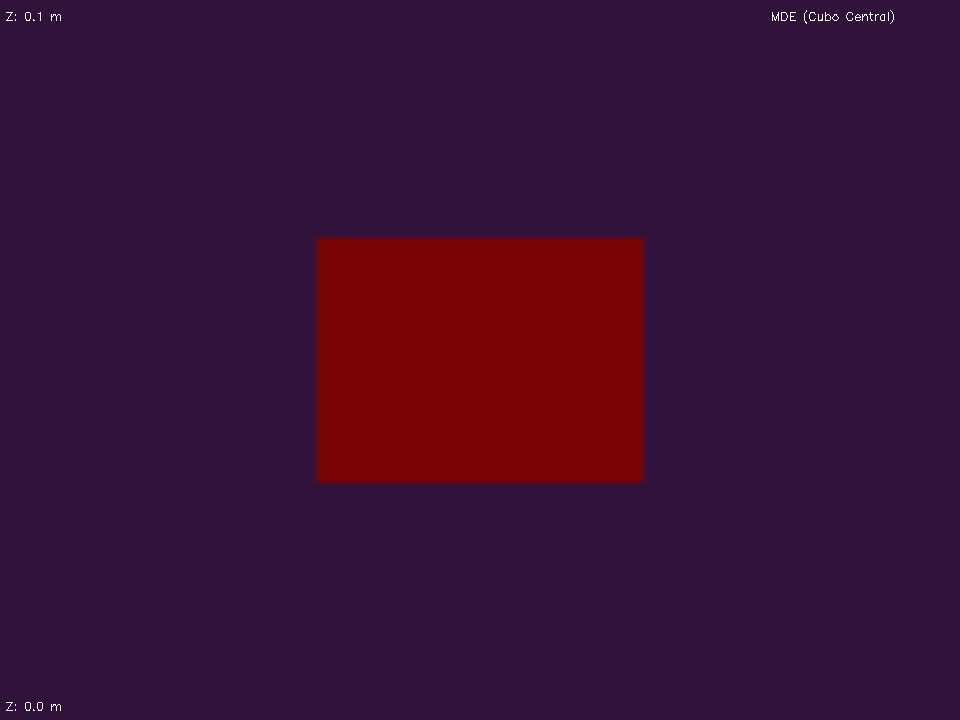
\includegraphics[width=0.7\textwidth]{img/gabarito_mde_cubo.png}
\caption{Janela \texttt{Gabarito\_MDE}: heatmap do MDE sintético Cubo
Central, com o HUD de estado no canto superior/inferior esquerdo.}
\label{fig:gabarito-cubo}
\end{figure}

\begin{figure}[!ht]
\centering
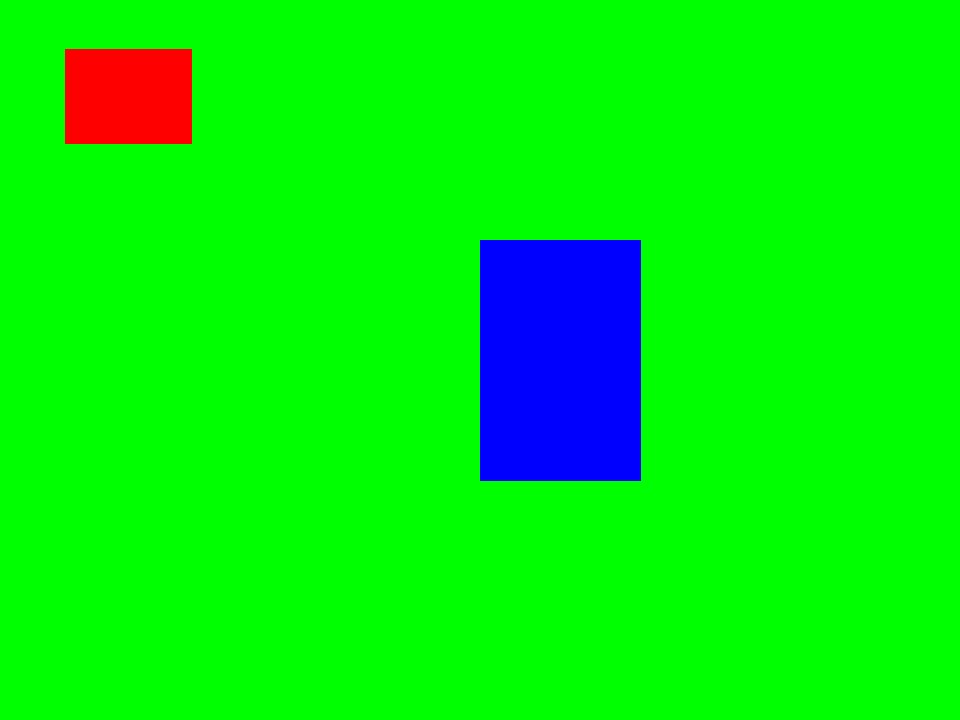
\includegraphics[width=0.7\textwidth]{img/projecao_areia_cubo.png}
\caption{Janela \texttt{Projecao\_Areia}: malha discretizada renderizada
pelo \textit{pipeline} completo (\texttt{gerar\_imagem\_grade\_cores}),
em um estágio intermediário de modelagem — verde (correto), azul
(falta areia) e vermelho (excesso) simultaneamente visíveis.}
\label{fig:projecao-cubo}
\end{figure}

A taxa de quadros medida em uma máquina típica de desenvolvimento
(Intel i5 de oitava geração, 8~GiB de RAM, sem GPU dedicada) supera
30~fps de forma consistente, resposta mais que suficiente
para interação humana fluida.

\subsection{Modo real}

Em modo real, com o sensor Kinect~v2 (adaptado, Seção~\ref{cap:rendering})
conectado via USB~3.0, o sistema processa nuvens de até
$512 \times 424 = 217{.}088$ pontos brutos por \textit{frame}, reduzidos
pelo filtro de alcance ($0{,}5$ a $4{,}5$~m) e, após a calibração, pelo
filtro \texttt{dentro} do domínio físico da mesa
(Seção~\ref{subsec:T-shift}). A taxa de quadros de $>30$~fps reportada
para o modo simulação (Seção anterior) não foi remedida de forma
independente em modo real: os ensaios de campo confirmaram resposta
visual fluida ao vivo, mas sem um número de FPS especificamente
registrado nessas condições. Como as etapas computacionalmente
dominantes do \textit{pipeline} — discretização em malha e rasterização
— são idênticas nos dois modos, e a única diferença é a origem da nuvem
de pontos (chamada à API do Kinect \textit{versus} leitura de um
\texttt{array} em memória), não há razão matemática para esperar
degradação relevante; ainda assim, um número medido e reportado seria
uma evidência mais forte do que essa inferência, e sua obtenção fica
registrada como item pendente para trabalhos futuros
(Seção~\ref{sec:trabalhos-futuros}).

A calibração oficial (RANSAC + SVD,
Seção~\ref{sec:passo1}) foi exercitada repetidamente ao longo de
sucessivos ensaios de campo com o sensor físico conectado, em que a
tampa de calibração era reposicionada e a rotina de calibração
disparada pela tecla \texttt{C}; a validação de sanidade da distância
sensor--plano (tolerância de 15~cm) mostrou-se eficaz para sinalizar
tampas mal posicionadas antes que uma calibração incorreta fosse
persistida em \texttt{calibration\_data.json}. Esses ensaios com
hardware real — e não apenas a suíte sintética de testes unitários —
foram o que expôs originalmente o defeito de calibração descrito na
Seção~\ref{sec:correcao}, posteriormente reproduzido de forma
determinística pelo teste de aceitação (Seção~\ref{sec:aceitacao}) para
evitar regressões. Vale registrar, com total transparência, que a
demonstração física completa e ininterrupta do roteiro de aceitação
(Apêndice~A) não foi plenamente concluída nos ensaios finais, por
causas físicas/operacionais — instabilidade da conexão USB do sensor e
oclusão parcial da câmera pela estrutura do caixão de teste — discutidas
em detalhe, junto da evidência independente que sustenta a corretude
do \textit{software} mesmo diante dessa limitação, na
Seção~\ref{subsec:limitacao-fisica}.

\section{Defeito Detectado e Correção Implementada}
\label{sec:correcao}

Durante o ensaio preliminar de campo, foi observado um defeito visual
significativo: após a calibração com o sensor apontado para uma
superfície plana (piso de concreto), a janela \texttt{Projecao\_Areia}
exibia apenas um pequeno retângulo azul no canto inferior, em
vez da malha contínua esperada de quadrados coloridos. A
Figura~\ref{fig:bug} ilustra o sintoma observado.

\begin{figure}[!ht]
\centering
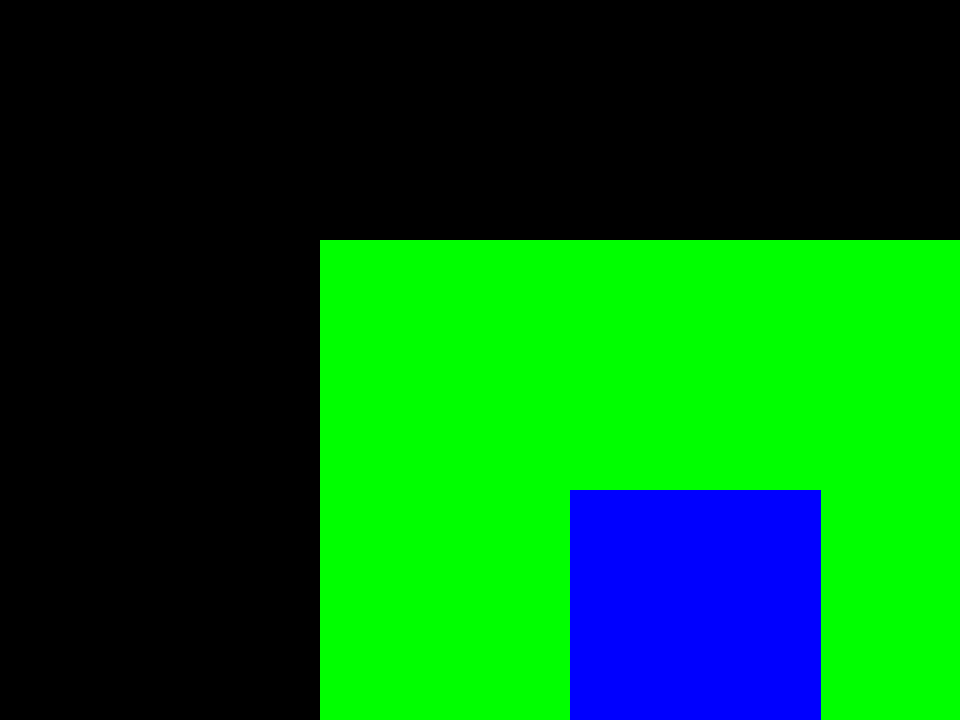
\includegraphics[width=0.7\textwidth]{img/bug_calibracao.png}
\caption{Reconstituição do defeito de calibração (versão 3.0), obtida
executando o próprio \textit{pipeline} de renderização de produção
(\texttt{gerar\_imagem\_grade\_cores}) com os parâmetros \textit{mock}
de projetor então usados em modo real ($f_x = f_y = 500$,
$c_x = 320$, $c_y = 240$, $\mathbf{t}_{\text{ext}} = (0,0,1)^{T}$):
apenas uma fração da janela é preenchida pela malha, o restante
permanece preto. Não é a captura de tela original do incidente de
campo, que não foi preservada — é uma reprodução fiel do mecanismo do
defeito a partir dos parâmetros documentados na versão~3.0 do código.}
\label{fig:bug}
\end{figure}

\subsection{Diagnóstico}

A análise da implementação revelou duas causas concorrentes:

\begin{enumerate}
    \item A função \texttt{transformar\_pontos()}, ao aplicar a matriz
          $T$ obtida pela calibração, leva o centroide do plano à
          origem $(0, 0, 0)$. Em consequência, a nuvem
          transformada ocupa aproximadamente
          $[-L_x/2, +L_x/2] \times [-L_y/2, +L_y/2]$, e metade dos
          pontos possui coordenadas negativas. A função
          \texttt{discretizar\_nuvem\_em\_grade()} aplicava
          \texttt{numpy.clip} nos índices de célula, colapsando todos
          esses pontos negativos na coluna~0 e na linha~0 da grade —
          isto é, em uma estreita faixa de borda;
    \item Os parâmetros de projeção do projetor, em modo real, eram
          valores \textit{mock} de placeholder ($f_x = f_y = 500$,
          $c_x = 320$, $c_y = 240$, $\mathbf{t}_{\text{ext}} = (0,0,1)^{T}$),
          que mapeavam o domínio da mesa para uma sub-região da janela
          em vez de preenchê-la integralmente.
\end{enumerate}

\subsection{Correção implementada}

A correção, materializada na versão~3.1 do sistema, contemplou três
ajustes simultâneos em \texttt{main.py} e \texttt{motor\_caixao\_areia.py}:

\begin{enumerate}
    \item \textbf{Composição com $T_{\text{shift}}$.} A matriz de
          transformação final é agora $T_{\text{final}} = T_{\text{shift}}
          \cdot T$, conforme a Equação~\eqref{eq:T-shift}, o que desloca
          o centroide ao centro lógico $(L_x/2, L_y/2)$ da mesa;
    \item \textbf{Filtro \texttt{dentro}.} A função
          \texttt{discretizar\_nuvem\_em\_grade()} passou a descartar
          pontos com $x \notin [0, L_x)$ ou $y \notin [0, L_y)$ antes do
          \texttt{clip}, eliminando o acúmulo nas células de borda;
    \item \textbf{Projeção coerente.} Os parâmetros do projetor
          em modo real foram substituídos pela mesma parametrização
          empregada na simulação (Equação~\eqref{eq:fxfy-virtual}),
          assegurando que a malha preencha a janela integralmente.
\end{enumerate}

\noindent As três alterações foram testadas em conjunto — em ensaios
de campo pontuais com o sensor real e, de forma determinística e
repetível, pelo teste de aceitação (Seção~\ref{sec:aceitacao}) — e o
defeito visual aqui descrito não voltou a se manifestar; essa
conclusão refere-se especificamente a este defeito, e não deve ser
confundida com a conclusão do roteiro de demonstração completo de
onze passos, cuja execução ininterrupta com hardware real é discutida
separadamente na Seção~\ref{subsec:limitacao-fisica}. A suíte de testes unitários permanece
integralmente válida após as correções, pois nenhum dos contratos
matemáticos das funções afetadas foi alterado — somente a composição
foi adicionada no nível do orquestrador.

\section{Discussão de \emph{Trade-offs}}
\label{sec:tradeoffs}

\subsection{Resolução da malha}

A escolha de $30 \times 30$ células (5~cm$\,\times\,$5~cm cada) é o
equilíbrio entre quatro fatores:

\begin{itemize}
    \item \textbf{Granularidade visual.} Células maiores tornam a
          imagem ``grosseira'' e perdem detalhe topográfico;
    \item \textbf{Filtragem de ruído.} Células menores recebem menos
          pontos por unidade, comprometendo a redução $\sigma/\sqrt{n}$
          do ruído de profundidade;
    \item \textbf{Custo de renderização.} O número de chamadas a
          \texttt{cv2.fillPoly} é $N_x \cdot N_y$, escalando
          quadraticamente com a resolução;
    \item \textbf{Significado militar.} Em escala 1:50~000 (carta
          tática típica), 5~cm na mesa equivalem a 2,5~km no terreno —
          uma resolução compatível com a granularidade operacional.
\end{itemize}

\subsection{Tolerância de cor}

A tolerância $\tau = 0{,}02$~m (2~cm) foi escolhida considerando
duas grandezas: o ruído residual após a agregação espacial
($\sigma_{\bar{Z}} \lesssim 1$~mm para dezenas de pontos por célula) e
a granularidade prática da operação manual humana com areia (uma mão
desloca naturalmente entre 1 e 3~cm por movimento). Valores menores
produziriam oscilações visuais perceptíveis durante o trabalho; valores
maiores reduziriam a precisão final do terreno modelado.

\subsection{Linguagem e \emph{stack}}

A escolha de Python como linguagem principal é justificada pelo
ecossistema científico maduro (NumPy, SciPy, OpenCV), pela velocidade
de desenvolvimento e pela facilidade de inspeção em ambiente
acadêmico. As operações computacionalmente intensivas — SVD,
back-projection, projeção de Tsai, rasterização — são integralmente
delegadas a rotinas em C/C++ via NumPy e OpenCV, eliminando o gargalo
do interpretador.

% =====================================================================
% conclusao.tex — Conclusão e Trabalhos Futuros
% =====================================================================

\chapter{Conclusão}
\label{cap:conclusao}

\section{Síntese das Contribuições}

Este Projeto Final de Curso apresentou o desenvolvimento integral de
um sistema de Caixão de Areia com Realidade Aumentada para apoio ao
treinamento militar em operações no terreno. O sistema combina,
de maneira engenhosa, três elementos centrais: (i) o rigor matemático
de uma calibração geométrica completa baseada em SVD, Gram-Schmidt e
modelo \textit{pinhole} de Tsai; (ii) a regra de negócio quantitativa
de comparação célula a célula contra um Modelo Digital de Elevação
fornecido em formato GeoTIFF, com tolerância vertical explícita; e
(iii) uma arquitetura resiliente, dotada de cadeia de
\textit{fallback} em quatro níveis, que assegura execução
\textit{plug and play} mesmo na ausência total de hardware ou de
dados cartográficos.

O motor matemático foi desenvolvido sob a metodologia de
\textit{Test-Driven Development}, resultando em uma suíte com 88
testes unitários automatizados que verificam — com valores numéricos
explícitos e auditáveis — todos os contratos algébricos do sistema,
da calibração RANSAC + SVD ao teste de aceitação de ponta a ponta.
A arquitetura monolítica modularizada, com seus quatro padrões de
projeto (Strategy + Fallback, Adapter, State Machine, Observer),
garante simultaneamente a latência mínima necessária para operação
em tempo real e a separação clara de responsabilidades indispensável
à manutenção.

A renderização por malha discretizada — em substituição à projeção
ingênua de pontos isolados — produz \textit{feedback} visual
contínuo, geometricamente preciso, computacionalmente eficiente e
estatisticamente robusto ao ruído do sensor. O emulador interativo
controlado por \emph{mouse} permite, em qualquer máquina sem hardware
especializado, demonstrar todo o \textit{pipeline} de forma tangível,
funcionalidade especialmente valiosa para defesa do projeto e para
ensino em sala de aula.

Durante a fase de validação em campo com o sensor Kinect~v2 real, foi
identificado e corrigido um defeito de calibração que reduzia a área
renderizada a uma pequena fração da janela de projeção. A correção,
formalizada na composição com a matriz $T_{\text{shift}}$ e na
introdução do filtro de extensão da mesa, foi documentada com
detalhes no Capítulo~\ref{cap:resultados} e permanece consolidada nas
versões subsequentes do sistema, que evoluíram a calibração para o
esquema RANSAC~+~SVD sobre uma superfície de referência (tampa ou
base vazia) com cota zero fixada na base do caixão.

\section{Atendimento aos Objetivos}

Todos os oito objetivos específicos enunciados no
Capítulo~\ref{cap:intro} foram atendidos:

\begin{enumerate}
    \item Arquitetura de três camadas implementada e documentada;
    \item Cadeia de \textit{fallback} do \texttt{KinectSensor} operacional;
    \item Motor matemático com SVD + Gram-Schmidt + Tsai funcional;
    \item \texttt{AdaptadorMDE} implementado, com \emph{fallback} gaussiano
          validado por teste automatizado; a leitura de GeoTIFF real está
          implementada e integrada ao restante do \textit{pipeline}, mas
          — como registrado com transparência na
          Seção~\ref{sec:tdd} — ainda não possui um caso de teste
          automatizado dedicado nem foi demonstrada com o arquivo
          \texttt{25S51\_ZN.tif} versionado no repositório, permanecendo
          como item de verificação futura (Seção~\ref{sec:trabalhos-futuros});
    \item Discretização em malha com renderização por \texttt{cv2.fillPoly};
    \item Emulador interativo via \texttt{cv2.setMouseCallback};
    \item Suíte de 88 testes unitários, todos aprovados;
    \item Documentação tripla (acadêmica, prática e relatório ABNT).
\end{enumerate}

\section{Trabalhos Futuros}
\label{sec:trabalhos-futuros}

A continuidade da linha de pesquisa pode explorar, dentre outras, as
seguintes frentes:

\begin{description}
    \item[Teste automatizado de leitura de GeoTIFF real.] A suíte atual
          valida a leitura de MDE apenas contra as superfícies
          sintéticas Cubo Central e Morro Gaussiano (Seção~\ref{sec:tdd}).
          Escrever um teste dedicado que carregue o GeoTIFF real já
          versionado no repositório (\texttt{25S51\_ZN.tif}) e valide a
          interpolação bilinear contra valores conhecidos da grade
          fecharia essa lacuna de cobertura.
    \item[Validação do erro quantitativo do MDE com ruído real de
          sensor.] O erro medido na Seção~\ref{subsec:erro-quantitativo-mde}
          (RMSE de 11,4\%) usa uma nuvem sintética livre de ruído — o
          único erro presente é a quantização geométrica da grade. O
          Kinect real introduz ruído próprio de profundidade,
          tipicamente mais acentuado nas bordas de objetos, que essa
          medição não captura; repetir a mesma análise com nuvens
          capturadas por hardware real, e para o mapa Morro Gaussiano
          além do Cubo Central, forneceria uma cota superior de erro
          mais realista.
    \item[Reconstrução do caixão de teste e nova demonstração física
          integral.] Corrigir o recorte da estrutura de madeira que
          hoje tampa parcialmente o campo de visão do sensor
          (Seção~\ref{subsec:limitacao-fisica}) e repetir o roteiro de
          aceitação completo com Kinect real, do início ao fim, sem
          interrupções de conexão.
    \item[Benchmark de desempenho em modo real.] Medir e reportar a
          taxa de quadros com o sensor Kinect conectado, de forma
          independente da medição já feita em modo simulação
          (Seção~\ref{sec:funcional}).
    \item[Calibração automática do projetor.] A versão atual emprega
          parâmetros de projeção configurados analiticamente. Uma
          calibração genuína do projetor por padrões \textit{Gray code}
          ou tabuleiro de xadrez (já parcialmente suportada pelas
          funções \texttt{encontrar\_\allowbreak cantos\_\allowbreak
          tabuleiro} e \texttt{calibrar\_\allowbreak projetor})
          eliminaria distorções residuais em montagens não-ideais.
    \item[Suporte a múltiplas camadas de visualização.] Sobreposição
          de curvas de nível, escalas batimétricas, isótermas e
          itinerários táticos — todos coerentes com o mesmo MDE de
          referência.
    \item[Integração com SARAS-FFT (Águas Pluviais).] Simulação
          hidrológica de escoamento sobre o relevo modelado, com
          renderização em tempo real do fluxo, em complemento à
          modelagem topográfica.
    \item[Substituição do Kinect por sensor moderno.] O Microsoft
          Kinect foi descontinuado; alternativas como o
          Intel RealSense, o Stereolabs ZED e o
          Microsoft Azure Kinect DK oferecem maior
          resolução e confiabilidade. A arquitetura
          \textit{strategy + fallback} já está preparada para
          acomodar essa migração com mínimo impacto.
    \item[Validação em escola militar.] Estudo experimental
          comparando o tempo médio de modelagem do terreno por
          turmas com e sem o sistema, e a fidelidade cartográfica
          do produto final medida por reconstrução fotogramétrica
          independente.
    \item[Exportação para realidade virtual.] A nuvem de pontos
          calibrada pode alimentar um \textit{viewer} VR (Oculus,
          HTC Vive) para imersão remota ou de instrução à distância.
\end{description}

\section{Considerações Finais}

A combinação de matemática rigorosa, engenharia de software
disciplinada e visão clara da aplicação militar produziu um sistema
que se diferencia das implementações de caixão de areia com realidade
aumentada de finalidade puramente didática ou recreativa levantadas na
revisão de trabalhos relacionados (Capítulo~\ref{cap:relacionados}),
por incorporar comparação quantitativa contra um MDE de referência,
tolerância vertical explícita e uma arquitetura de \textit{fallback}
resiliente. A entrega não se limita a um \textit{software} funcional: contempla
testes automatizados, documentação acadêmica completa, guia de uso
prático e este próprio relatório de conformidade ABNT, formando um
conjunto reproduzível, auditável e diretamente aproveitável pelas
escolas de formação militar.

Acreditamos que o trabalho contribui, ainda que modestamente, para
a tradição de excelência técnica do Instituto Militar de
Engenharia, e esperamos que sirva de ponto de partida para futuras
melhorias e adaptações por gerações seguintes de cadetes e
engenheiros militares.


% =========================================================
% POS-TEXTUAIS
% =========================================================
\postextual

\bibliography{refs}

\begin{apendicesenv}
    \partapendices
    % =====================================================================
% apendice.tex — Apêndice A: Roteiro de Demonstração
% =====================================================================

\chapter{Roteiro de Demonstração para a Banca}
\label{ap:roteiro}

Este apêndice consolida o roteiro de demonstração utilizado durante a
defesa do projeto, organizado em onze passos sequenciais que cobrem
desde a inicialização do sistema até a recalibração e o encerramento.
Cada passo é acompanhado da ação a ser executada e do resultado
esperado para fins de avaliação.

\begin{table}[!ht]
\centering
\caption{Roteiro de demonstração passo a passo.}
\label{tab:roteiro}
\small
\begin{tabularx}{\textwidth}{@{}c X X@{}}
\toprule
\textbf{\#} & \textbf{Ação} & \textbf{Resultado esperado} \\
\midrule
1  & Executar \texttt{python main.py}             & Abertura da GUI de configuração (CustomTkinter) \\
2  & Definir dimensões da mesa, modo de calibração (tampa/base) e mapa (GeoTIFF ou demo) & Janelas \texttt{Projecao\_Areia} e \texttt{Gabarito\_MDE} abertas \\
3  & Pressionar tecla \texttt{C}                  & Calibração executada (RANSAC + SVD + Gram-Schmidt + $T_{\text{shift}}$) \\
4  & Observar \texttt{Projecao\_Areia}            & Malha contínua: verde fora do cubo, azul no terço central (mapa Cubo Central) \\
5  & Observar \texttt{Gabarito\_MDE}              & Heatmap do MDE (Cubo Central, Morro Gaussiano ou GeoTIFF real) de referência \\
6  & Arrastar botão direito do mouse no terço central & Quadrados centrais transitam de azul $\to$ verde \\
7  & Arrastar botão esquerdo do mouse fora do cubo & Quadrados afetados transitam para azul, e voltam ao verde ao ajustar \\
8  & Continuar interação                          & Convergência da malha para totalmente verde \\
9  & Pressionar tecla \texttt{F}                  & Janela \texttt{Projecao\_Areia} entra em modo tela cheia \\
10 & Pressionar tecla \texttt{C} novamente        & Recalibração bem-sucedida (demonstra robustez) \\
11 & Pressionar tecla \texttt{Q} ou \texttt{ESC}  & Encerramento limpo, recursos liberados \\
\bottomrule
\end{tabularx}
\end{table}

\noindent
\textbf{Pontos-chave para destacar à banca:}
\begin{itemize}
    \item A interação com o \emph{mouse} demonstra em tempo real
          \emph{todo} o \textit{pipeline} matemático (discretização
          em malha $\to$ média espacial $\to$ comparação com MDE
          $\to$ projeção \textit{pinhole} de Tsai $\to$ rasterização
          por \texttt{cv2.fillPoly}), sem necessidade de
          hardware físico;
    \item A recalibração em tempo de execução comprova a robustez do
          mecanismo de \textit{fallback} e a estabilidade numérica do
          RANSAC seguido de SVD, mesmo após sucessivas modificações na
          areia virtual;
    \item A taxa de quadros (FPS) exibida no canto superior esquerdo
          da janela de projeção mantém-se consistentemente acima de
          30~fps, validando o requisito de operação em tempo real.
\end{itemize}

\section*{Comandos auxiliares}

Para executar a suíte de testes unitários:

\begin{lstlisting}
python -m unittest test_motor_caixao -v
\end{lstlisting}

\noindent Saída esperada: \texttt{88 passed}, com Open3D instalado.
Na ausência dessa biblioteca, o teste \texttt{TestLeituraRGBD} é
ignorado automaticamente, e a suíte reporta \texttt{87 passed} e
\texttt{1 skipped}.

Para forçar o modo simulação mesmo com Kinect conectado, editar no
topo do arquivo \texttt{main.py}:

\begin{lstlisting}
FORCAR_SIMULACAO = True
\end{lstlisting}

\end{apendicesenv}

\phantompart
\printindex

\end{document}
